%%%%%%%%%%%%%%%%%%%%%%%%%%%%%%%%%%%%%%%%%%%%%%%%%%%%%%%%%%%%%%%%%%%%%%%%%%%%%%%%%%%%%%%%%%%%%%%%%%%%%%%%%%%%%%%%%%%%%%%%%%%%%%%%%%%%%%%%%%%%%%%%%%%%%%%%%%%%%%%%%%%%%%%%%%%%%%%%%%%%
%%%%%%%%%%%%%%%%%%%%%%%%%%%%%%%%%%%%%%%%%%%%%%%%%%%%%%%%%%%%%%%%%%%%%%%%%%%%%%%%%%%%%%%%%%%%%%%%%%%%%%%%%%%%%%%%%%%%%%%%%%%%%%%%%%%%%%%%%%%%%%%%%%%%%%%%%%%%%%%%%%%%%%%%%%%%%%%%%%%%
\FloatBarrier
\chapter{Event selection}
\label{sec:EventSelection}
\section{Datasets and triggers}
\label{sec:DatasetsAndTriggers}

The analysis is performed on $pp$-collision data recorded in the year 2012 by the CMS experiment at a centre-of-mass energy of $\sqrt{s}=8\tev$.
In total an integrated luminosity of 19.7\fbinv was recorded in 2012.

As outlined in Section~\ref{sec:GeneralSearchStrategy}, the detection of chargino tracks is a challenging task already on trigger level.
Direct triggering of events containing chargino-like tracks is not possible because in 2012 there was no dedicated track trigger available.
Furthermore, there is no intrinsic missing transverse energy in the event if the chargino is not reconstructed as a PF particle, \eg when it decays inside the tracker.
Therefore, this analysis uses initial state radiation for the detection of chargino events.
If ISR occurs, it is possible to trigger on a high-\pt jet (\ptfirstjet) and missing transverse momentum (\met).

For this purpose, several triggers are utilised in this analysis.
An event is selected, if at least one of the three triggers in Table~\ref{tab:triggers} fired.
The \seqsplit{HLTMonoCentralPFJet80\_{PF}\-{MET}\-noMu95\_NHEF0p95} and HLTMonoCentralPFJet80\_PFMETnoMu105\_NHEF0p95 triggers both rely on the L1 ETM40 trigger which requires the missing energy to be larger than 40\gev.
On HLT level, they further require at least one particle-flow jet within the pseudorapidity range of $|\eta|<2.6$ with $\pt>80\gev$ and the PF missing transverse momentum (not taking into account the \pt of muons) to be larger than 95\gev or 105\gev, respectively.
Finally, no more than 95\% of the jet energy must be carried by neutral hadrons.
The HLTMonoCentralPFJet80\_PFMETnoMu95\_NHEF0p95 trigger was active during Run\,A and Run\,B in 2012 data taking, whereas HLTMonoCentralPFJet80\_PFMETnoMu105\_NHEF0p95 was in place during Run\,C and Run\,D in 2012.

\renewcommand{\arraystretch}{1.5}
\begin{table}[!t]
\centering
\caption{\met and \met+ jet triggers used in this analysis together with the corresponding recorded integrated luminosity during the time when they were in place.}
\label{tab:triggers}
\makebox[0.99\textwidth]{
\begin{tabular}{lr}
\multicolumn{2}{c}{} \\
\toprule
Trigger  & Integrated luminosity [\fbinv]   \\
\midrule
 HLTMonoCentralPFJet80\_PFMETnoMu95\_NHEF0p95     &  5.3   \\
 HLTMonoCentralPFJet80\_PFMETnoMu105\_NHEF0p95    &  14.4  \\
 HLT\_MET120\_HBHENoiseCleaned                    &  19.7  \\
\bottomrule
%\multicolumn{2}{c}{}
\end{tabular}}
\end{table}  

The HLT\_MET120\_HBHENoiseCleaned trigger is based on the L1 trigger ETM36. % that are combined by a logical OR.
On HLT level, the trigger requires that the missing energy measured from calorimeter energy deposits is larger than 120\gev.
The HBHENoise-filter reduces background from electronic noise in the HCAL.
This trigger was active during the full data taking period in 2012.

\renewcommand{\arraystretch}{1.5}
\begin{table}[!b]
\centering
\caption{MET data samples used in the search with the contained integrated \mbox{luminosity}.}
\label{tab:SearchSamples}
\makebox[0.99\textwidth]{
\begin{tabular}{lr}
\multicolumn{2}{c}{} \\
\toprule
Dataset  & Integrated luminosity [\fbinv]   \\
\midrule
 /MET/Run2012A-22Jan2013-v1/RECO         &  0.876   \\
 /MET/Run2012B-22Jan2013-v1/RECO         &  4.412  \\
 /MET/Run2012C-22Jan2013-v1/RECO         &  7.055  \\
 /METParked/Run2012D-22Jan2013-v1/RECO   &  7.354  \\ 
\bottomrule
%\multicolumn{2}{c}{}
\end{tabular}}
\end{table} 
The events that were selected by the described triggers are available in the MET datasets listed in Table~\ref{tab:SearchSamples}. 
Again, because of the size of the datasets ($\sim150\,$TB in total), a reduction of the size is achieved by selecting only events where one of the used triggers fires and that contains at least one jet with a minimum \pt of 50\gev.
This reduction in size of almost 80\% is necessary to make this analysis technically feasible.

%%%%%%%%%%%%%%%%%%%%%%%%%%%%%%%%%%%%%%%%%%%%%%%%%%%%%%%%%%%%%%%%%%%%%%%%%%%%%%%%%%%%%%%%%%%%%%%%%%%%%%%%%%%%%%%%%%%%%%%%%%%%%%%%%%%%%%%%%%%%%%%%%%%%%%%%%%%%%%%%%%%%%%%%%%%%%%%%%%%%
\section{Selection of signal candidate events}
\label{sec:AnalysisSelection}

In order to suppress events originating from Standard Model processes such as QCD-multijet events, \WJets, etc., a selection favouring signal-like tracks is applied.
The signal candidate selection closely follows the selection required in the disappearing track search~\cite{bib:CMS:DT_Thesis,bib:CMS:DT_8TeV_AN}.
It relies on event-based and track-based variables as described in the following two sections.


\subsection{Event-based selection}
\label{sec:EventBasedSelection}
First, a selection on the quality of the primary vertex is applied in order to suppress cosmic events and noise from the beam halo.
This selection includes requirements on the position of the vertex with respect to the beam axes and the number of degrees of freedom of the vertex which is strongly correlated to the number of tracks originating from the vertex (see~\cite{bib:CMS:Tracking_7TeV_PAS} for further details):  
\begin{itemize}
\renewcommand{\labelitemi}{\footnotesize{\ding{118}}}
\item The vertex must have at least four degrees of freedom: \mbox{$vtx$ with $\geq 4$ d.o.f.}
\item The position of the vertex along the beam line must be within 24\cm with respect to the nominal interaction point: \mbox{$|dz| \leq 24\cm$.}
\item The position in the transverse direction must be within 2\cm with respect to the nominal interaction point: \mbox{$|d0| \leq 2\cm$.}\\
\end{itemize}

To maximise the signal acceptance, the trigger related selection cuts are chosen close to the trigger thresholds (see Section~\ref{sec:DatasetsAndTriggers}).
In Fig.~\ref{fig:SignalMET+SignalJetPt}, the distributions of \met and the transverse momentum of the leading jet, \ptfirstjet, are shown for different signal models.
\begin{figure}[!t]
  \centering 
  \begin{tabular}{c}
    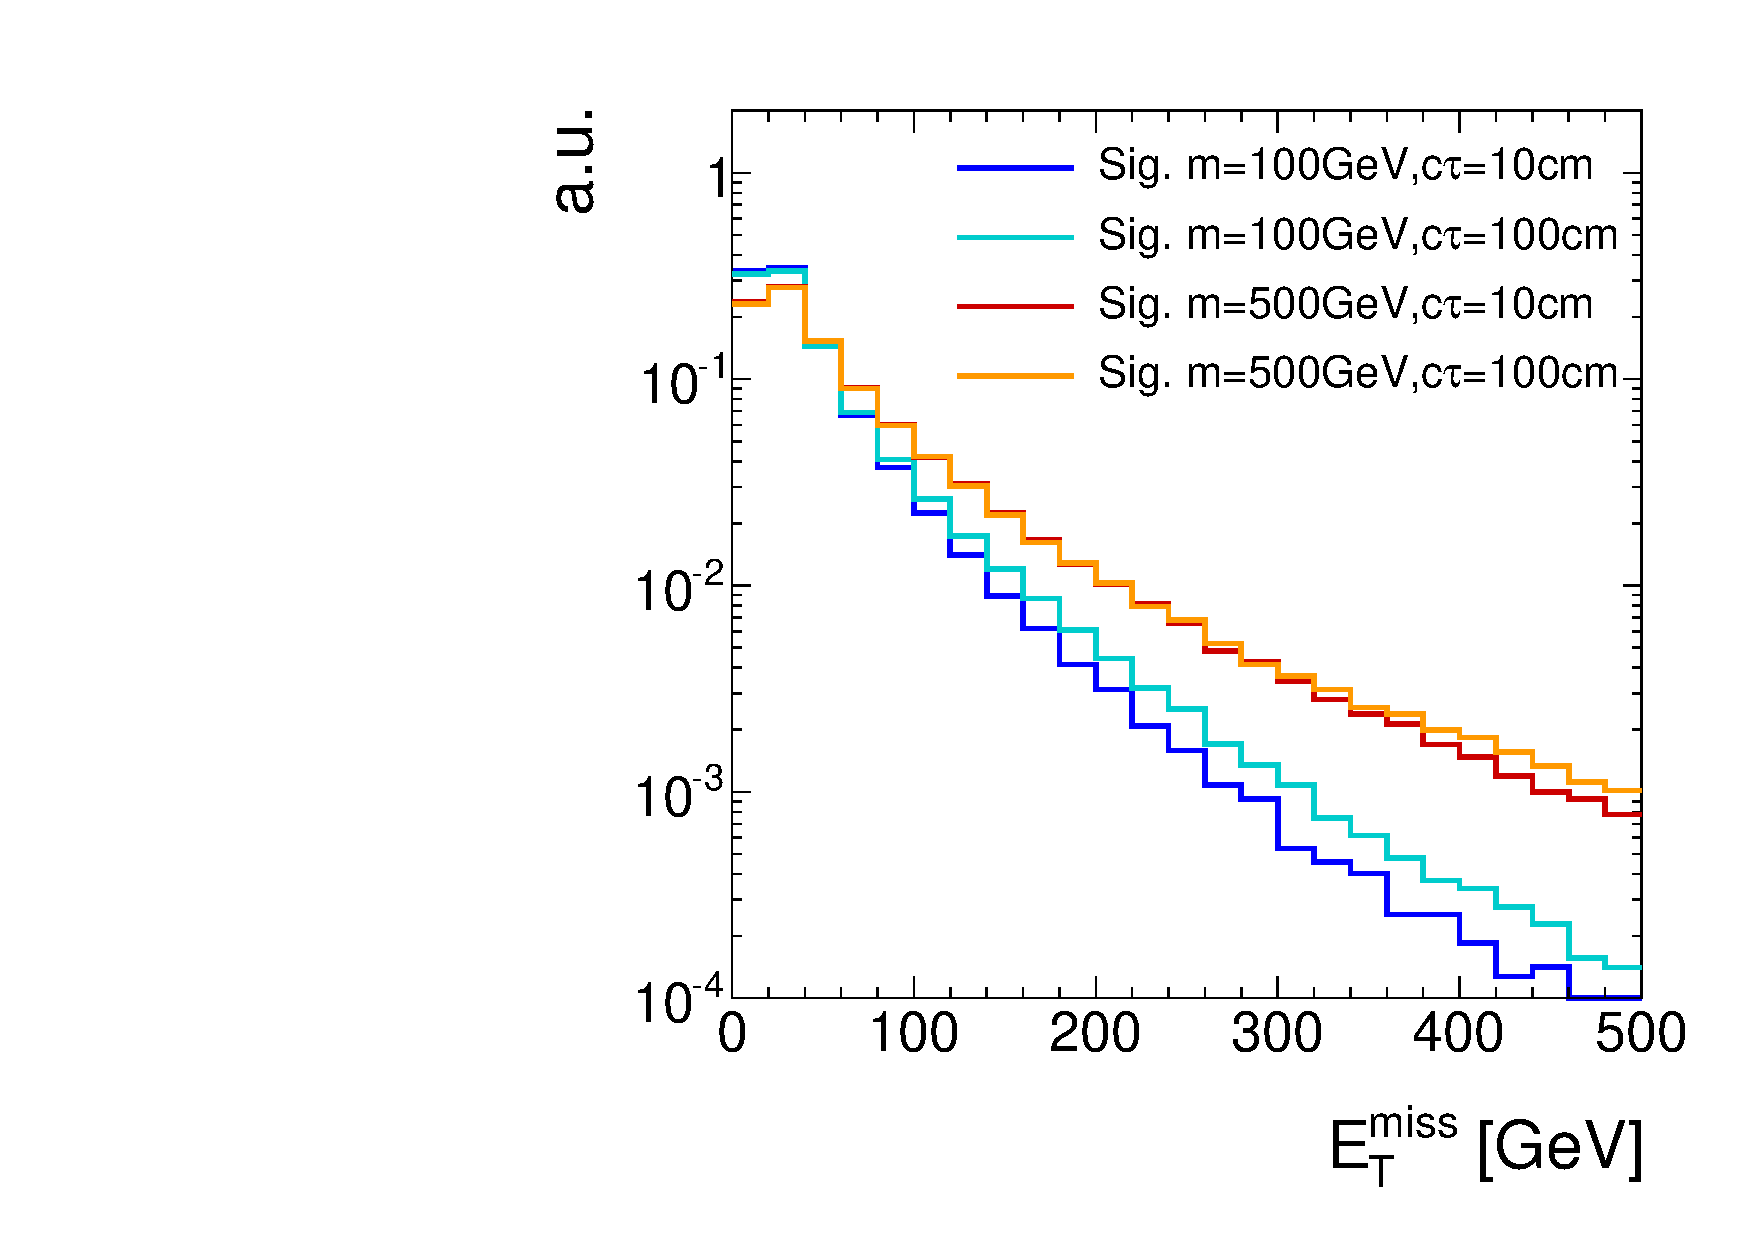
\includegraphics[width=0.49\textwidth]{figures/analysis/AnalysisSelection/hMetSmallRange_log_chiTracksnoSelection_4Signals.pdf}
    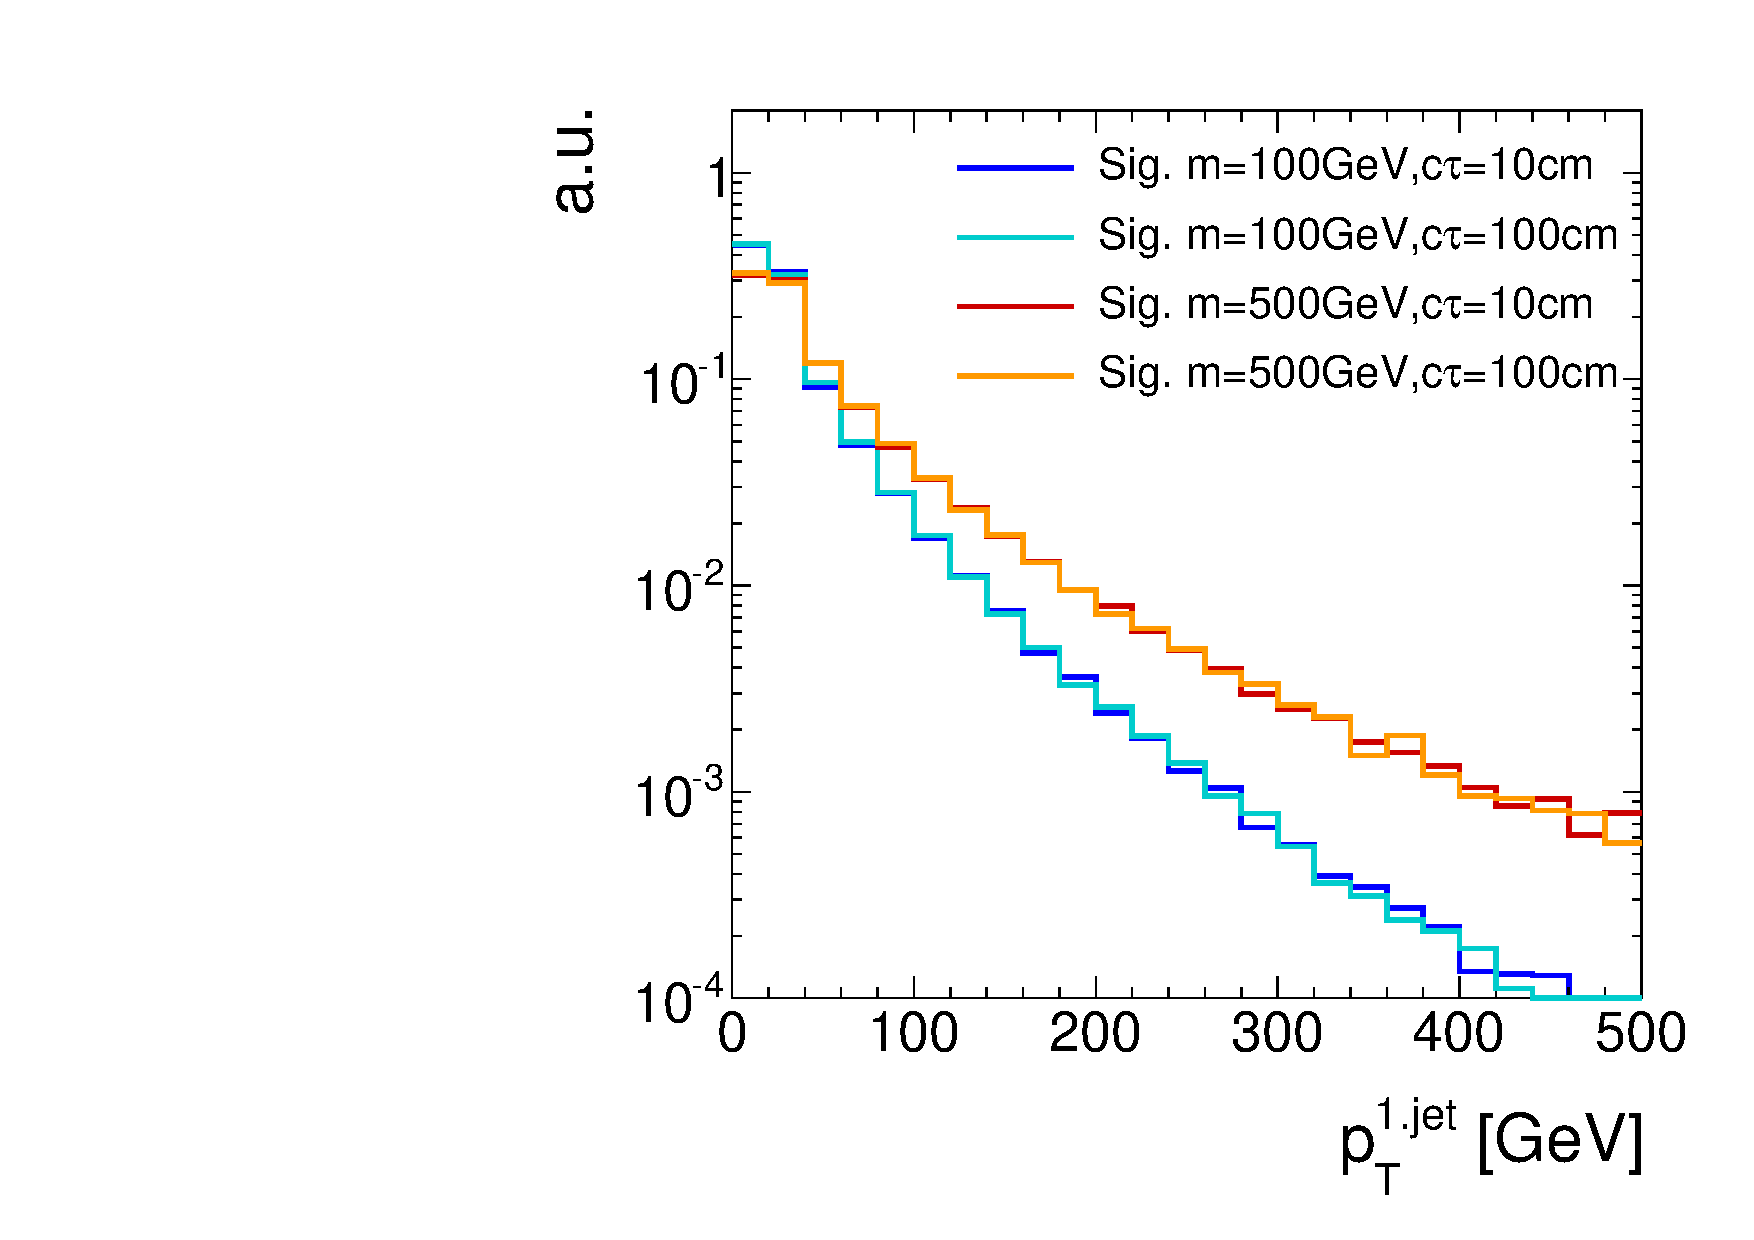
\includegraphics[width=0.49\textwidth]{figures/analysis/AnalysisSelection/h1stjetptSmallRange_log_chiTracksnoSelection_4Signals.pdf}
  \end{tabular}
  \caption{Normalised distributions of the missing transverse momentum (left) and the transverse momentum of the leading jet (right) for four different signal models.}
  \label{fig:SignalMET+SignalJetPt}
\end{figure}
The leading jet has to be centrally produced, $|\eta_{\text{\nth{1}jet}}|<2.4$, and to fulfil the following criteria: %Only jets with $|\eta|<2.4$ that fulfil the following further criteria are taken into account:
\begin{itemize}
\item Charged hadron energy fraction (CHF$_{\text{\nth{1}jet}}$) $>0.2$
\item Charged electromagnetic energy fraction (CEF$_{\text{\nth{1}jet}}$) $<0.5$
\item Neutral hadron energy fraction (NHF$_{\text{\nth{1}jet}}$) $<0.7$
\item Neutral electromagnetic energy fraction (NEF$_{\text{\nth{1}jet}}$) $<0.7$.
\end{itemize}
These additional jet quality criteria ensure that noise from cosmic and beam halo muons and high-\pt photons and electrons is suppressed \cite{bib:CMS:DM_8TeV_AN}.

The trigger efficiency as a function of \met and \ptfirstjet was determined within~\cite{bib:CMS:DM_8TeV} with a single-muon reference sample.
The trigger paths become fully efficient for $\ptfirstjet \gtrsim 110\gev$ and $\met \gtrsim 220\gev$~\cite{bib:CMS:DM_8TeV_AN}.
However, it can be seen in Fig.~\ref{fig:SignalMET+SignalJetPt} that for a selection of \mbox{$\met>220\gev$} more than 99\% of the signal events are rejected.

In order to achieve a reasonable signal acceptance, this search imposes, therefore, a trigger selection closer to the intrinsic trigger thresholds.
The trigger selection is as follows:
\begin{itemize}
\renewcommand{\labelitemi}{\footnotesize{\ding{118}}}
\item There is at least one jet within $|\eta|<2.4$ with transverse momentum larger than 110\gev which fulfils the above mentioned jet noise cleaning criteria: \mbox{$\ptfirstjet>110\gev$}.
\item The missing transverse momentum must be larger than 100\gev: \mbox{$\met>100\gev$}
\end{itemize}
These requirements result in an efficiency of 100\% for the trigger requirements on the jet \pt and an efficiency of $\sim5-20\%$ for the trigger requirement on \met, at the \met thresholds~\cite{bib:CMS:DM_8TeV_AN}.
Throughout the following sections, these trigger related requirements will be referred to as ``trigger selection''.\\  %in the variable \ptfirstjet and $\sim20\%$ in the variable \met at the cut thresholds~\cite{bib:CMS:DM_8TeV_AN}.\\

Because of the huge cross section, QCD-multijet events are frequently produced at the LHC.
Due to jet energy mismeasurements, they can also contribute to data samples recorded with MET triggers.
Therefore, special requirements are enforced in order to suppress events emerging from QCD-multijet processes.
QCD-multijet events can be characterised by topologies where two jets are almost back-to back.
Additionally, in QCD-multijet events the missing energy is usually aligned with one of the leading jets in the event.
Figure~\ref{fig:QCDcuts} shows the maximum $\Delta\phi$ of any of two jets ($\pt>20\gev, |\eta|<4.5$) and the minimum $\Delta\phi$ between the \met vector and any of the two leading jets for the SM background and two different signal datasets.
\begin{figure}[!t]
  \centering 
  \begin{tabular}{c}
    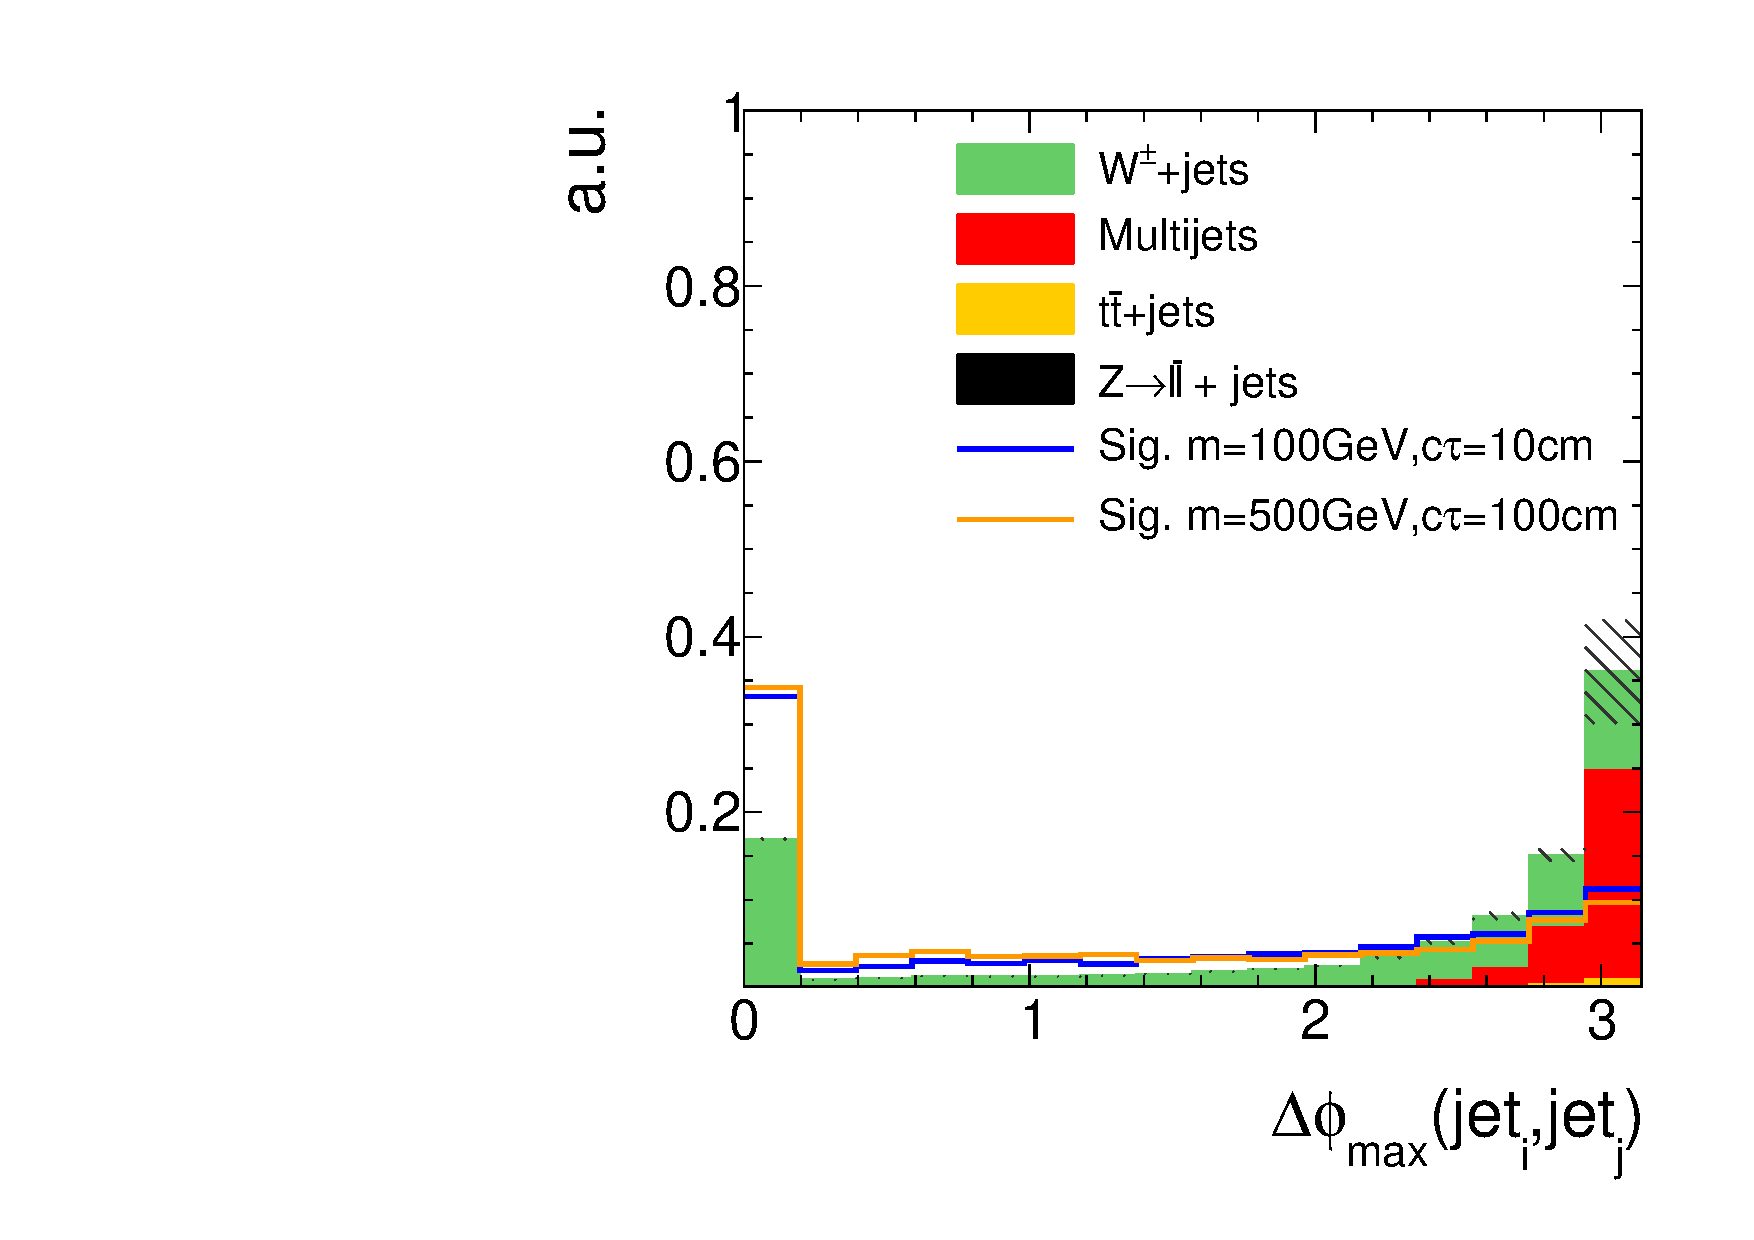
\includegraphics[width=0.49\textwidth]{figures/analysis/AnalysisSelection/chiTrackstriggerRequirementsTrigger_2Signals_FullBkg/hDeltaPhiMaxbeforeCut_lin.pdf}
    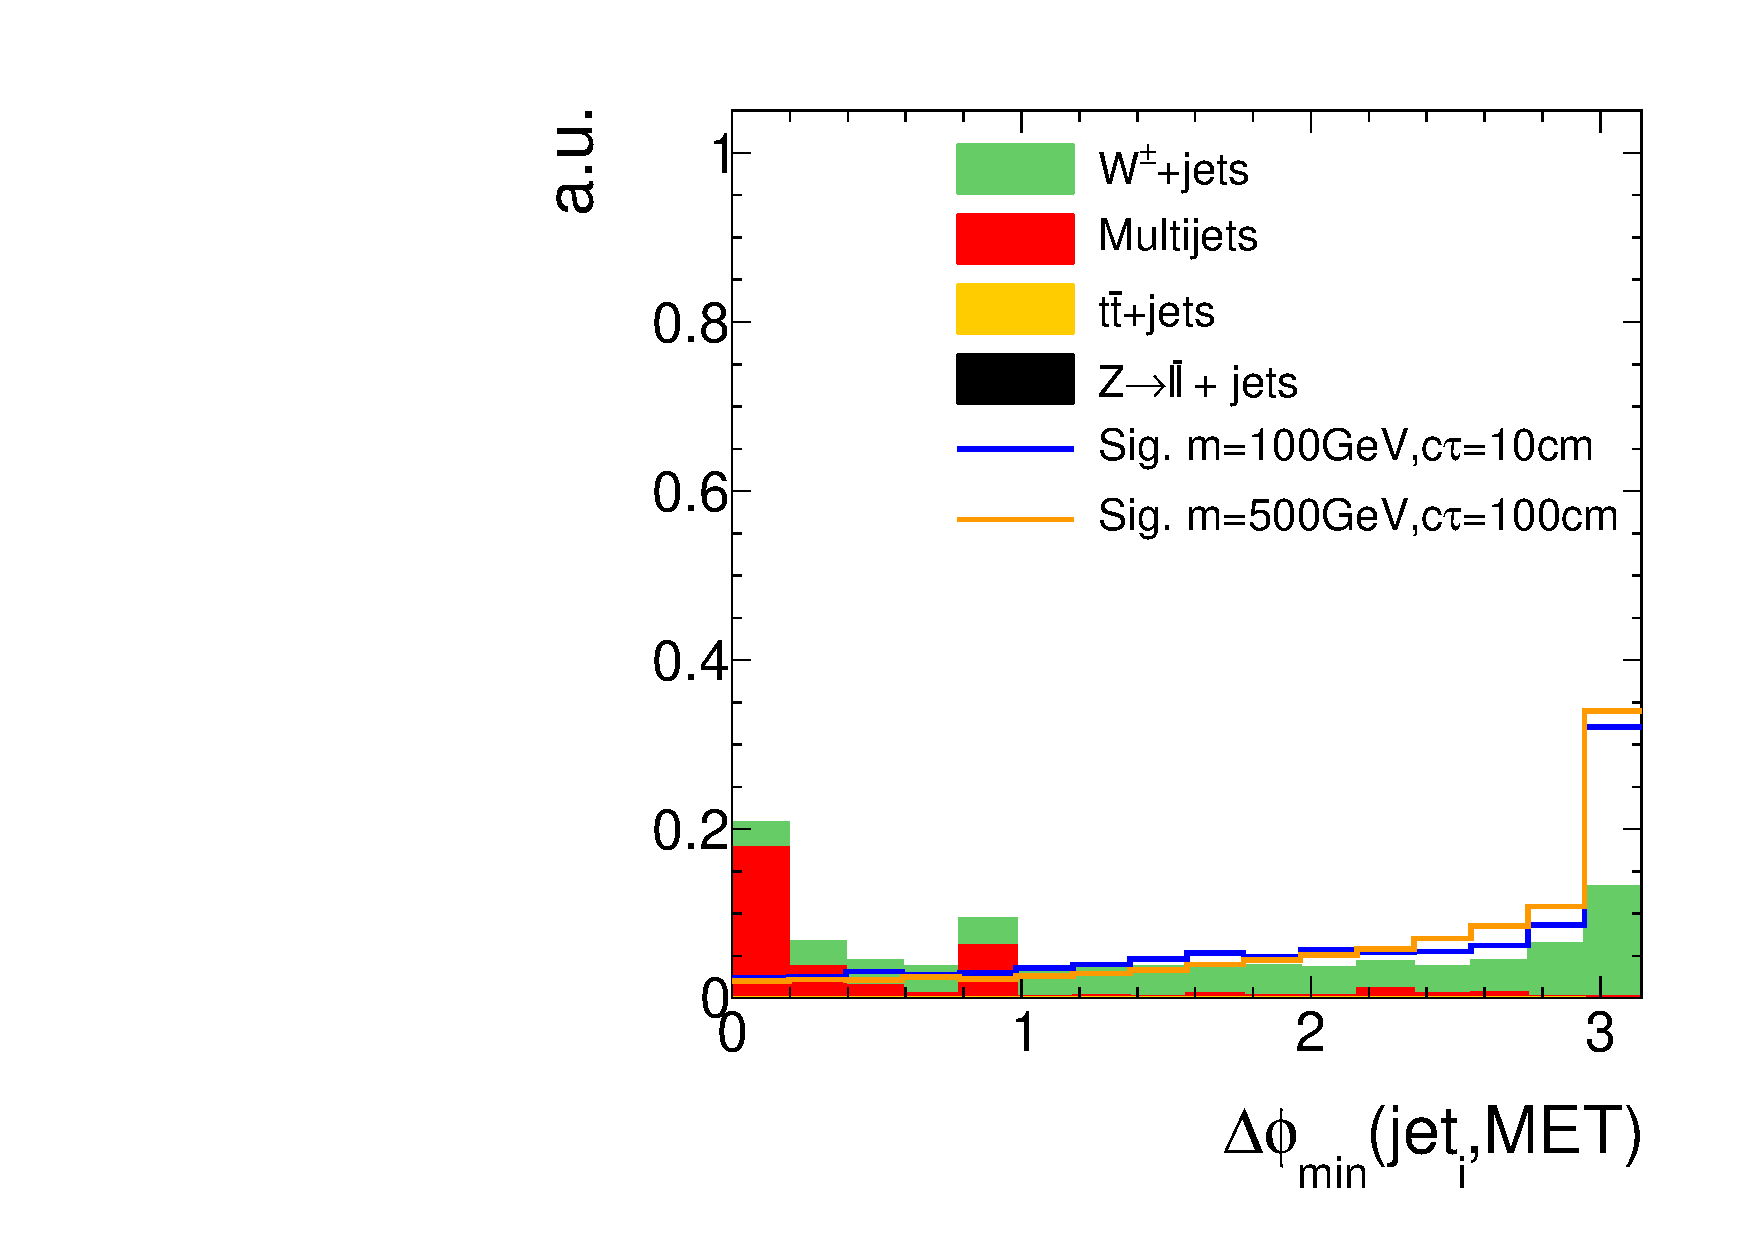
\includegraphics[width=0.49\textwidth]{figures/analysis/AnalysisSelection/chiTrackstriggerRequirementsTrigger_2Signals_FullBkg/hDeltaPhiJetMetMinbeforeCut_lin.pdf}
  \end{tabular}
  \caption{Maximum $\Delta \phi$ between any of two jets (left) and the minimum $\Delta \phi$  between the \met vector and any of the two leading jets (right) normalised to unit area after trigger selection.
           Only jets with $\pt>20\gev$ and $|\eta|<4.5$ are considered.}
  \label{fig:QCDcuts}
\end{figure}

The following two requirements are sufficient to suppress QCD-multijet events efficiently:
\begin{itemize}
\renewcommand{\labelitemi}{\footnotesize{\ding{118}}}
\item $\Delta\phi$ between any of two jets (with $\pt>20\gev$ and $|\eta|<4.5$) in the event must be smaller than 2.5. %: \mbox{$\Delta\phi\left( j_i, j_j\right)<2.5$}.
\item $\Delta\phi$ between any of the two leading jets (with $\pt>20\gev$ and $|\eta|<4.5$) and the \met must be larger than 0.5. %: \mbox{$\Delta\phi\left( j_{1,2}, \metvec \right) > 0.5$.} 
\end{itemize}



\subsection{Candidate track selection}
\label{sec:CandidateTrackSelection}
After the reduction of background processes with event-based variables, a track-based selection is carried out.
To get an optimised selection for possible chargino tracks several signal candidate track characteristics are exploited.\\

First, a selection of high-quality tracks is enforced:
\begin{itemize}
\renewcommand{\labelitemi}{\footnotesize{\ding{118}}}
\item The track must be classified as ``high purity'' as defined in~\cite{bib:CMS:Tracking_2010}.
\item The track is required to have no missing middle or inner hits: $N_{\text{miss}}^{\text{middle/inner}}=0$
\item The radial and longitudinal  distance of the track to the primary vertex must be small: \mbox{$|d0|<0.02\cm$}, \mbox{$|dz|<0.5\cm$}.
\end{itemize}
In Figs.~\ref{fig:LostHits} and~\ref{fig:d0_dz}, the power of the latter two quality selection cuts is shown.
\begin{figure}[!h]
  \centering 
\vspace{20pt}
  \begin{tabular}{c}
    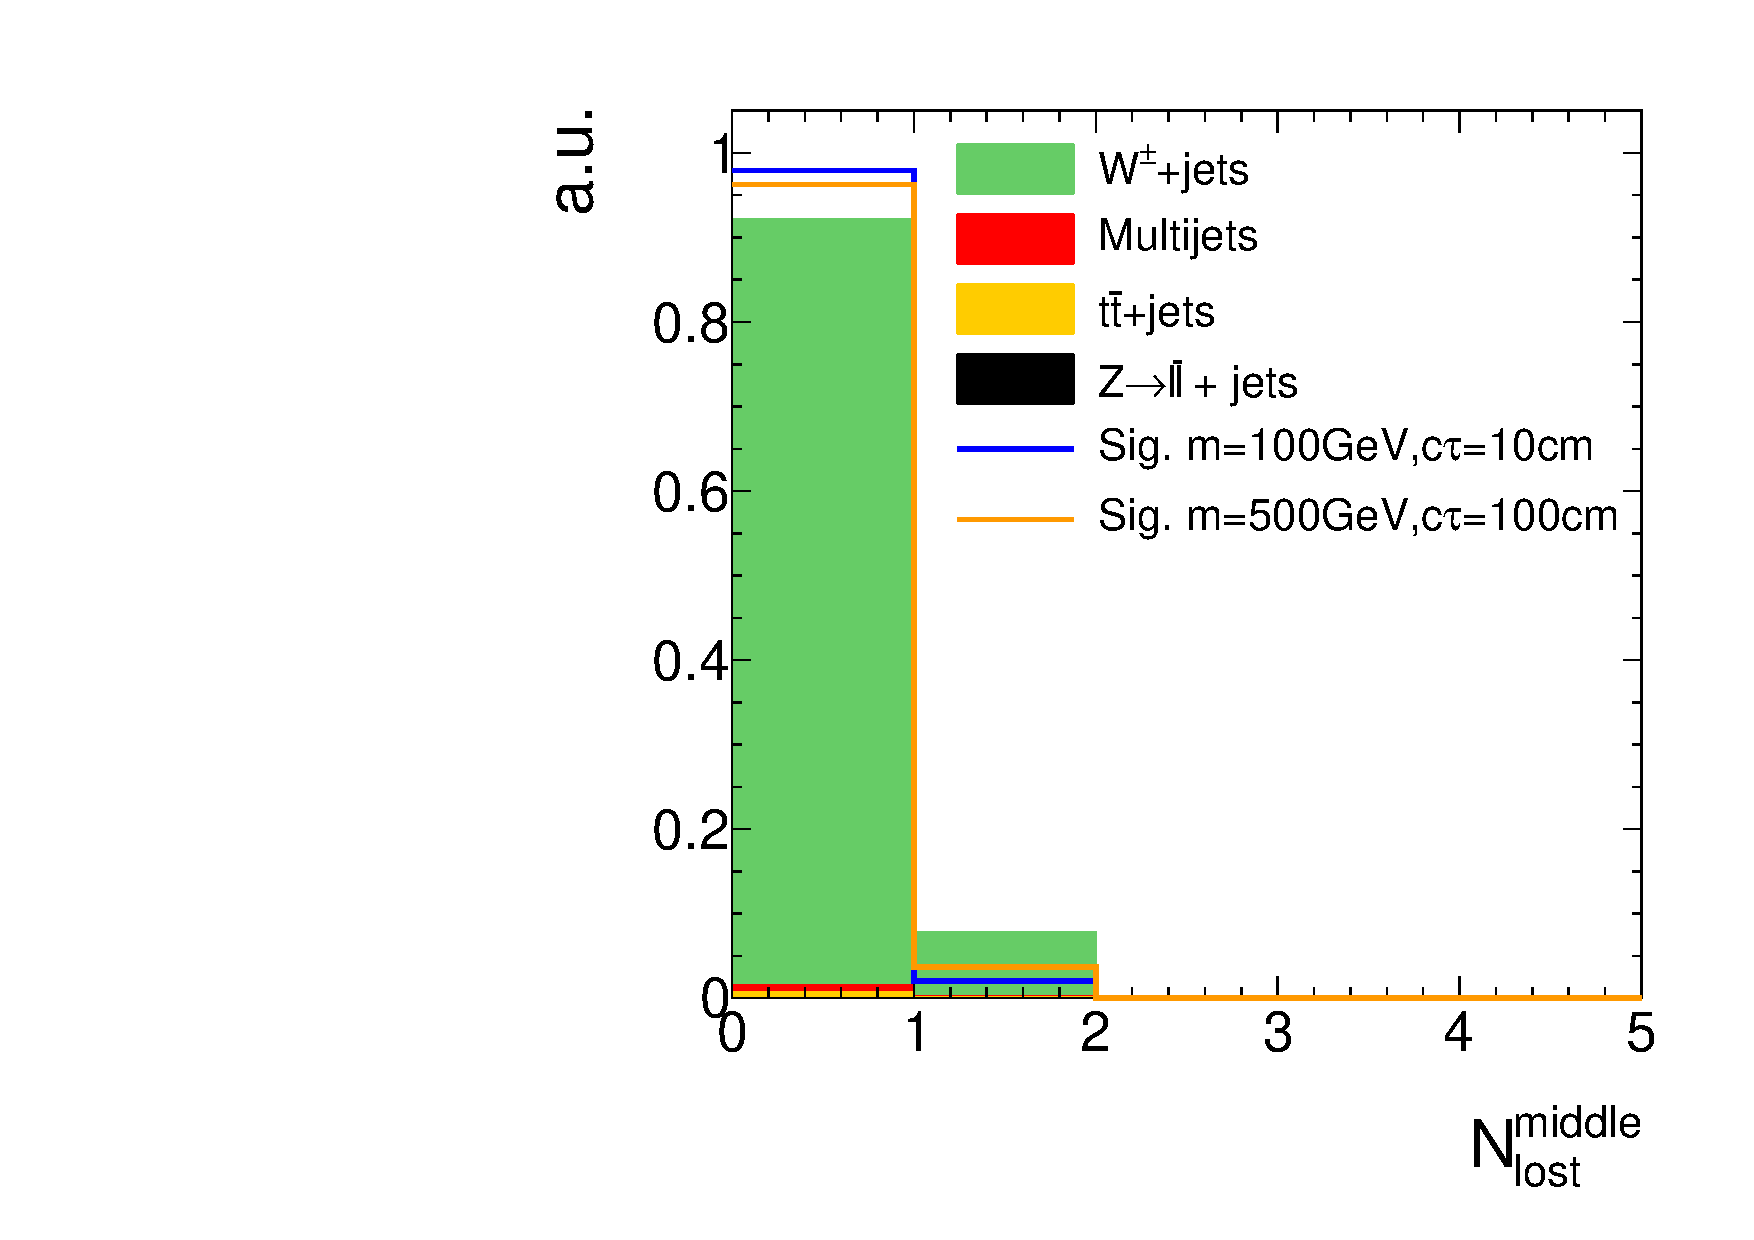
\includegraphics[width=0.49\textwidth]{figures/analysis/AnalysisSelection/chiTracksQCDsupressionTrigger_2Signals_FullBkg/htrackNLostMid_lin.pdf}
    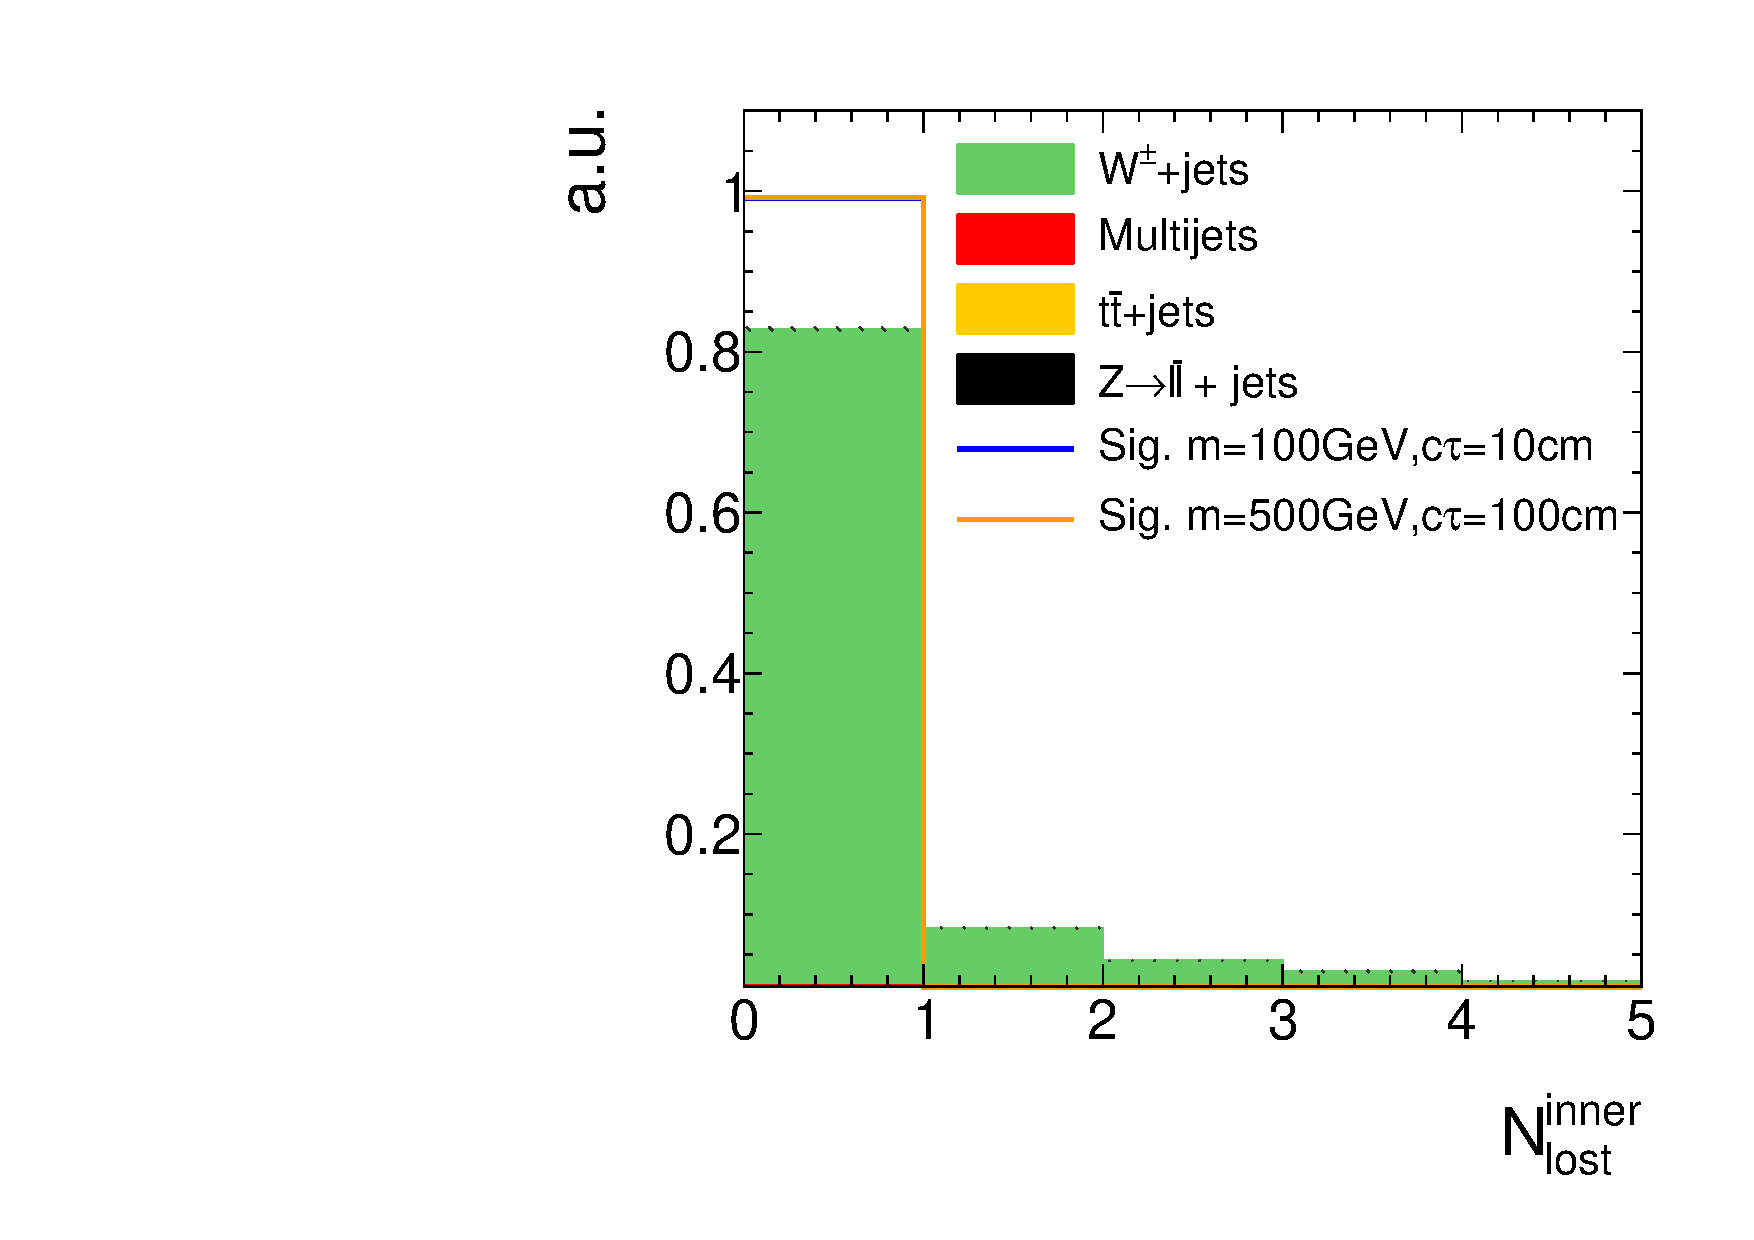
\includegraphics[width=0.49\textwidth]{figures/analysis/AnalysisSelection/chiTracksQCDsupressionTrigger_2Signals_FullBkg/htrackNLostInner_lin.pdf}
  \end{tabular}
  \caption{Normalised number of missing middle (left) and inner (right) hits of background and signal tracks after trigger selection and QCD suppression cuts (a.u. refers to normalised number of events).}
  \label{fig:LostHits}
\end{figure}
\begin{figure}[!h]
  \centering 
  \begin{tabular}{c}
    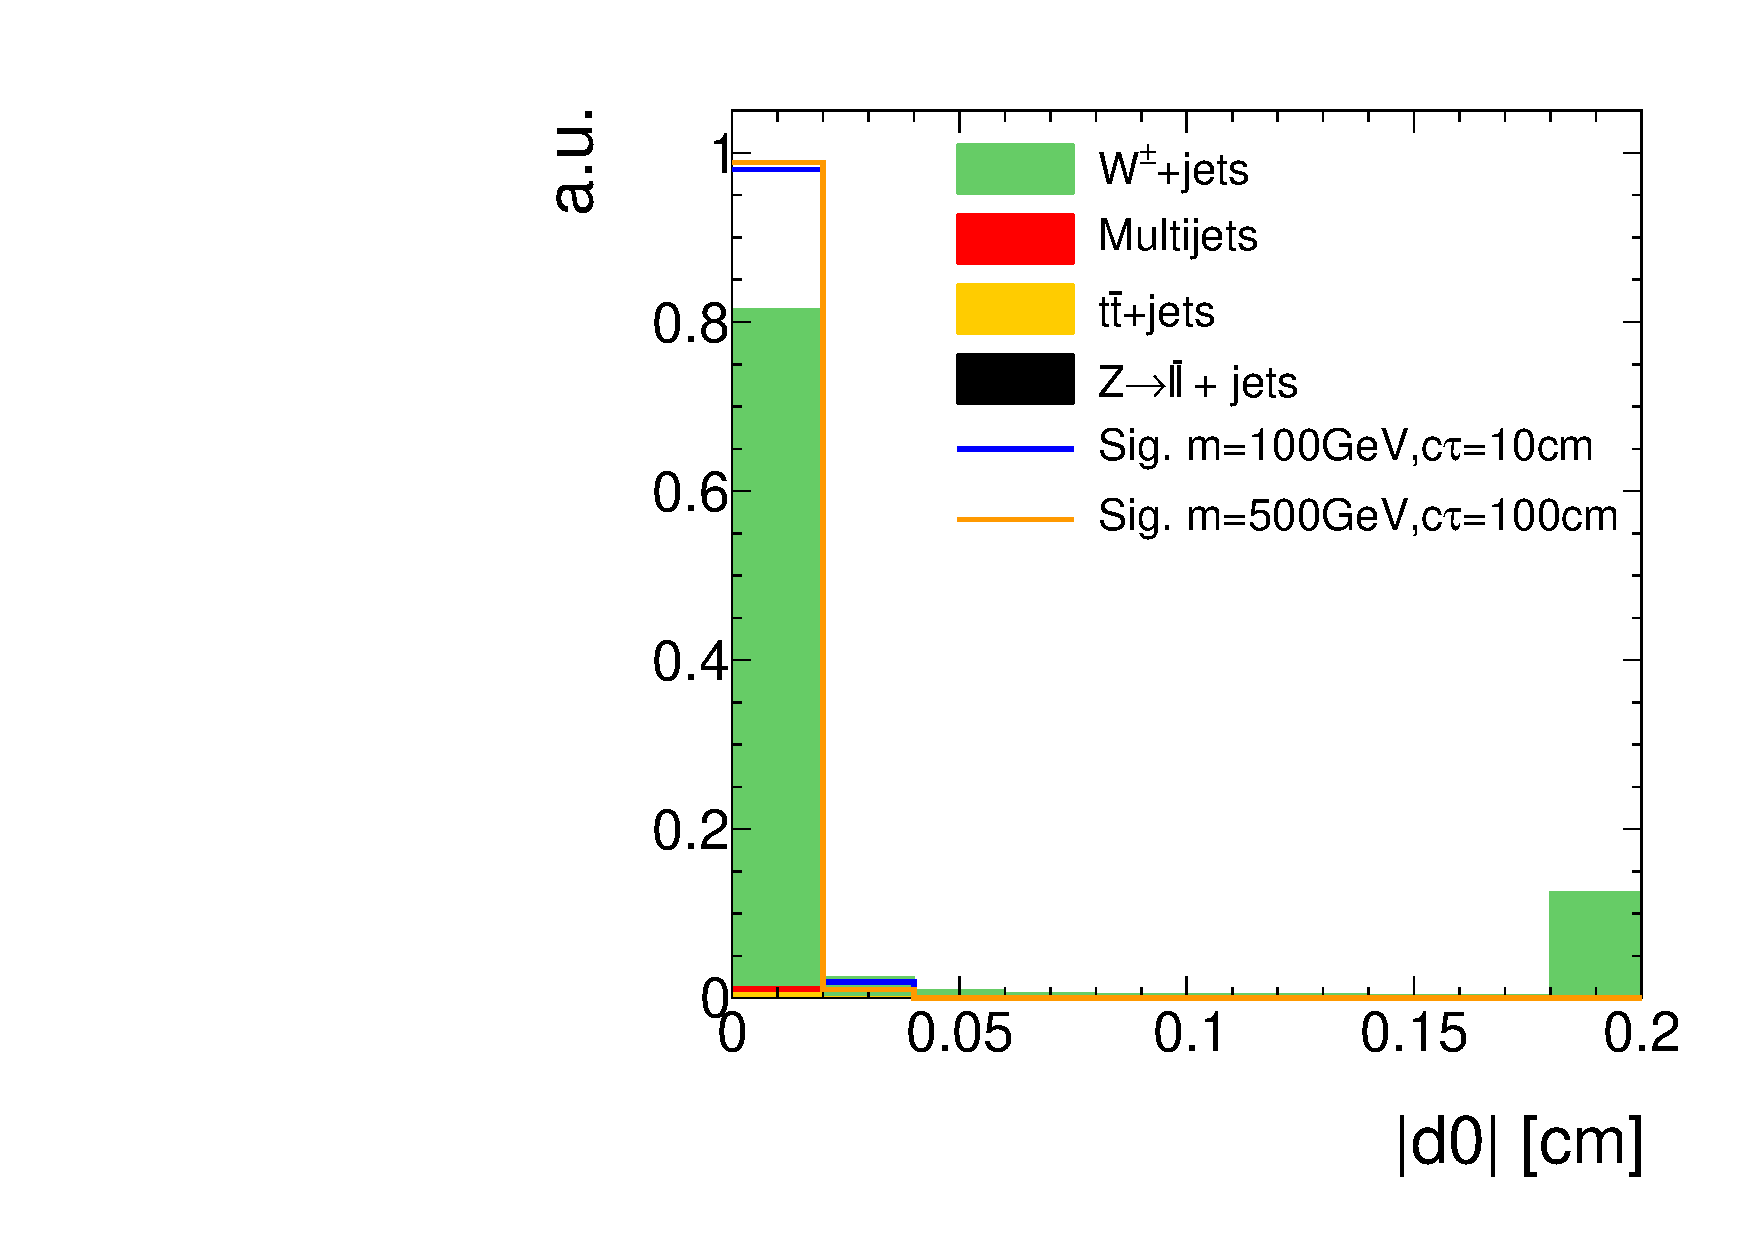
\includegraphics[width=0.49\textwidth]{figures/analysis/AnalysisSelection/chiTracksQCDsupressionTrigger_2Signals_FullBkg/htrackd0_lin.pdf}
    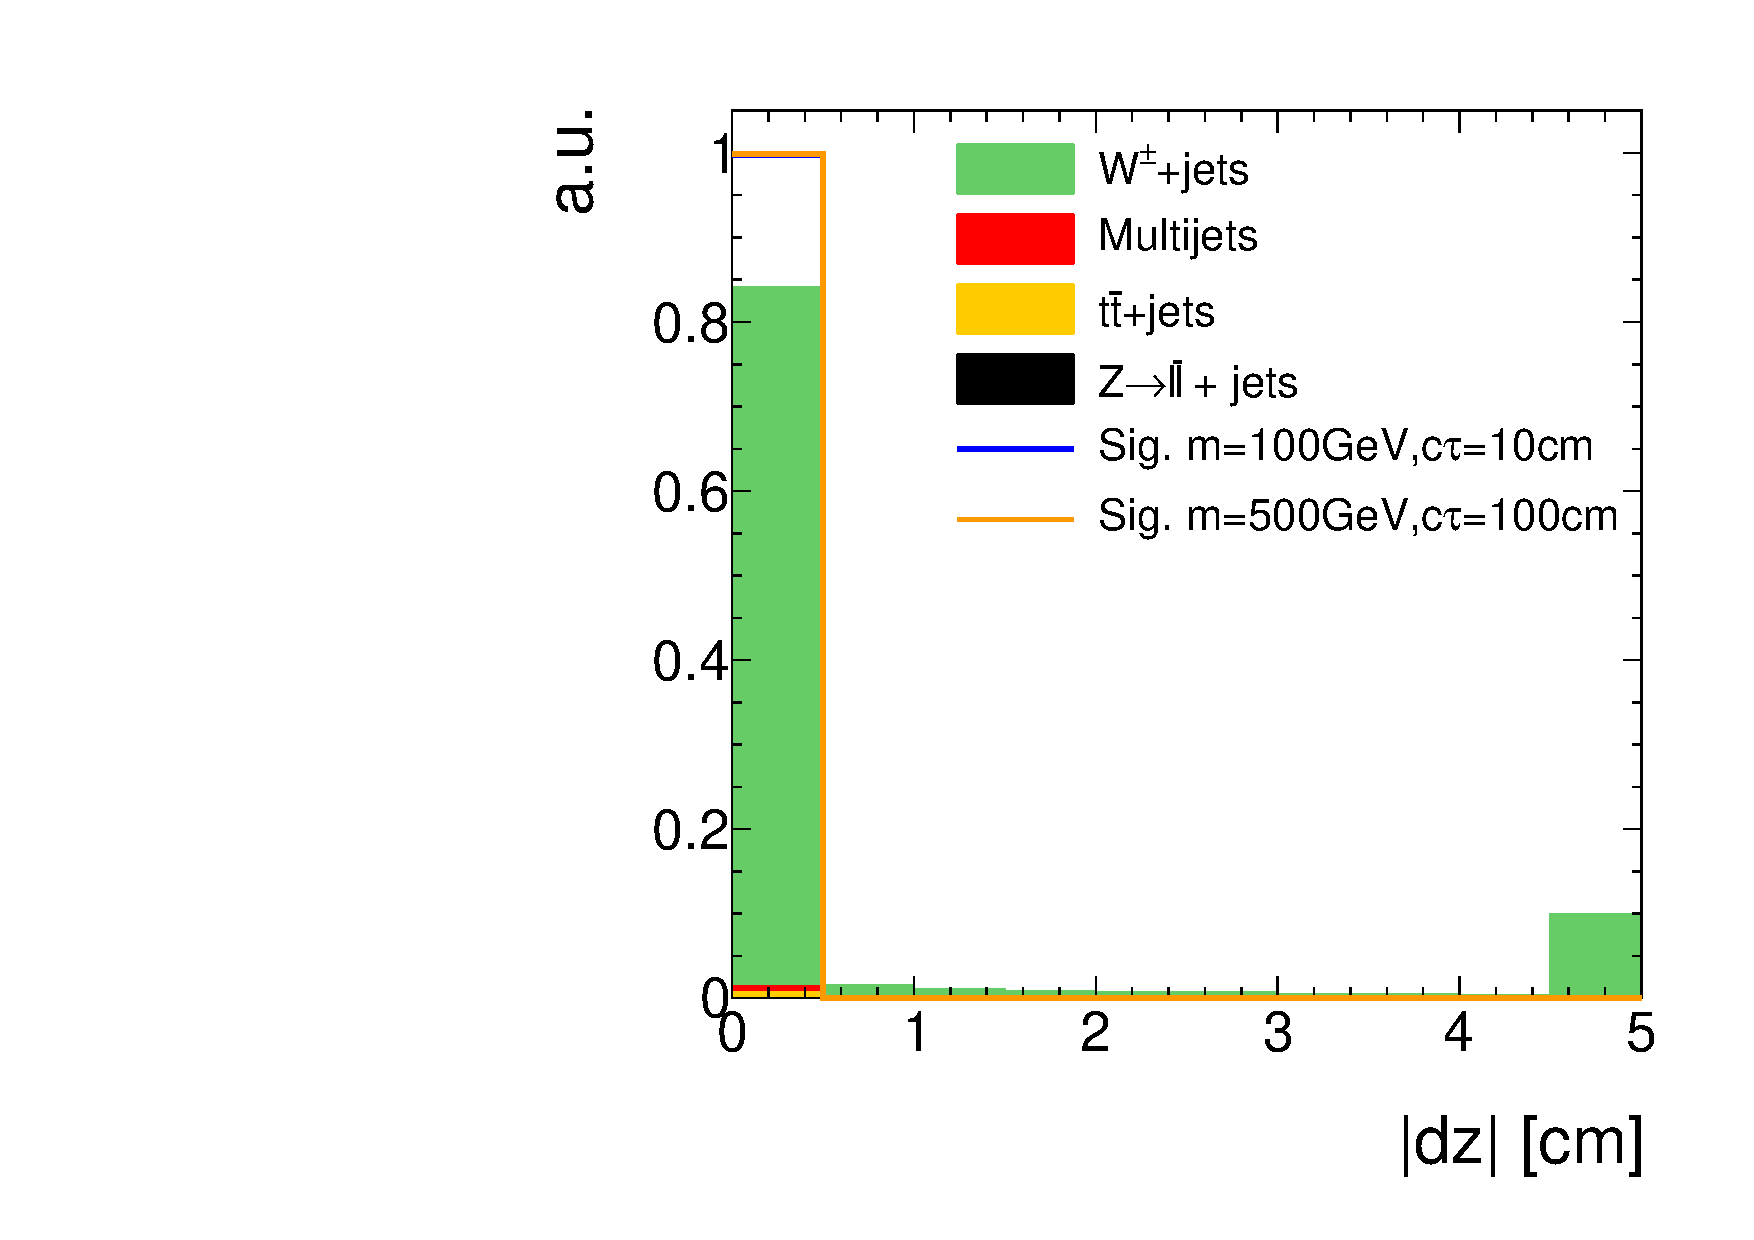
\includegraphics[width=0.49\textwidth]{figures/analysis/AnalysisSelection/chiTracksQCDsupressionTrigger_2Signals_FullBkg/htrackdz_lin.pdf}
  \end{tabular}
  \caption{Absolute value of the radial (left) and longitudinal (right) distance between the track and the primary vertex after trigger selection and QCD-multijet suppression cuts. 
           All events with a candidate track with a radial (longitudinal) distance larger than 0.2\cm (5\cm) are contained in the last bin.}
  \label{fig:d0_dz}
\vspace{20pt}
\end{figure}
\newpage
Furthermore, a first kinematic preselection is applied:
\begin{itemize}
\renewcommand{\labelitemi}{\footnotesize{\ding{118}}}
\item Only tracks in the central region are considered : $|\eta|<2.1$.
\item Only tracks with a minimum transverse momentum of 20\gev are considered:\\
       \mbox{$\pt>20\gev$}.\\
\end{itemize}
%\hspace{0.7cm}
%%%%%%%%%%%%%%%%%%%%%%%%%%%%%%%%%%%%%%%%%%%%%%%%%%%%%%%%%%%%%%%%%%%%%%%%

In order to suppress background tracks emerging from SM processes, an electron, muon and tau veto is applied.
This rejects tracks that are close to a reconstructed electron, muon or tau.
Additionally, the candidate track must not be close to a jet ($\pt>20\gev$ and $|\eta|<4.5$):
\begin{itemize}
\renewcommand{\labelitemi}{\footnotesize{\ding{118}}}
\item The track must not be within a cone of $\Delta R<0.15$ to a reconstructed standalone, tracker or global muon with a transverse momentum larger than 10\gev (see Section~\ref{subsec:MuonReconstruction} for details on the different muon definitions).
\item The track must not be within a cone of $\Delta R<0.15$ to a reconstructed electron with a transverse momentum larger than 10\gev (see Section~\ref{subsec:ElectronReconstruction} for details on the electron reconstruction).
\item The track must not be within a cone of $\Delta R<0.15$ to a reconstructed tau with $\pt>20\gev$ and $|\eta|<2.3$ (see Section~\ref{subsec:TauReconstruction} for details on the tau reconstruction). 
      Some loose isolation requirements are enforced to protect the tau reconstruction from jet contamination.
\item The track must not be within a cone of $\Delta R< 0.5$ to a reconstructed jet ($\pt>20\gev$ and $|\eta|<4.5$).\\
\end{itemize}
These lepton and jet veto selection requirements are highly suppressing the background emerging from real lepton/jet production like in \WJets events.
The discrimination power of the lepton and jet vetos is shown in Fig.~\ref{fig:TrackdRmin} where the minimum $\Delta R$ between the candidate track and a reconstructed electron, muon, tau or jet is shown.\\
\begin{figure}[!b]
  \centering 
  \vspace{25pt}
  \begin{tabular}{c}
    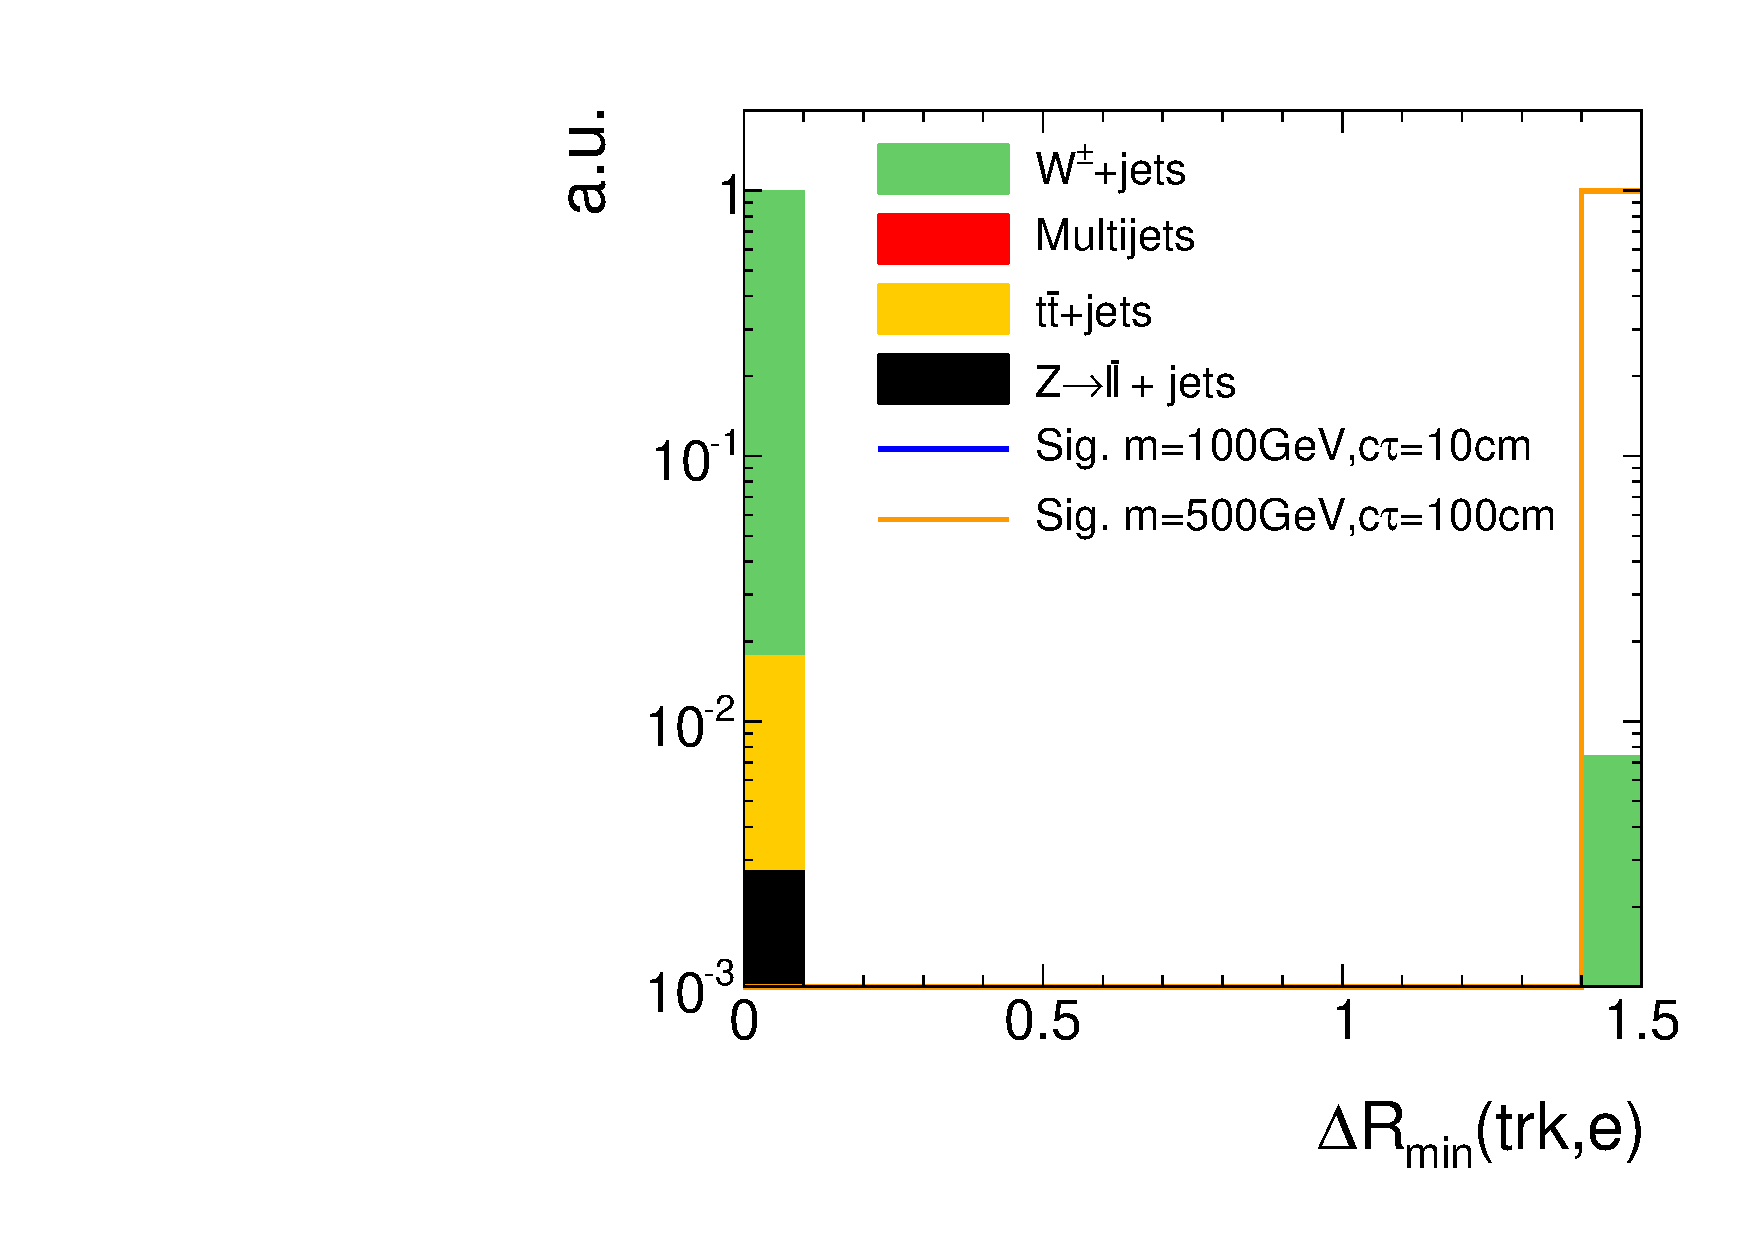
\includegraphics[width=0.49\textwidth]{figures/analysis/AnalysisSelection/htrackdRminElec_log.pdf}
    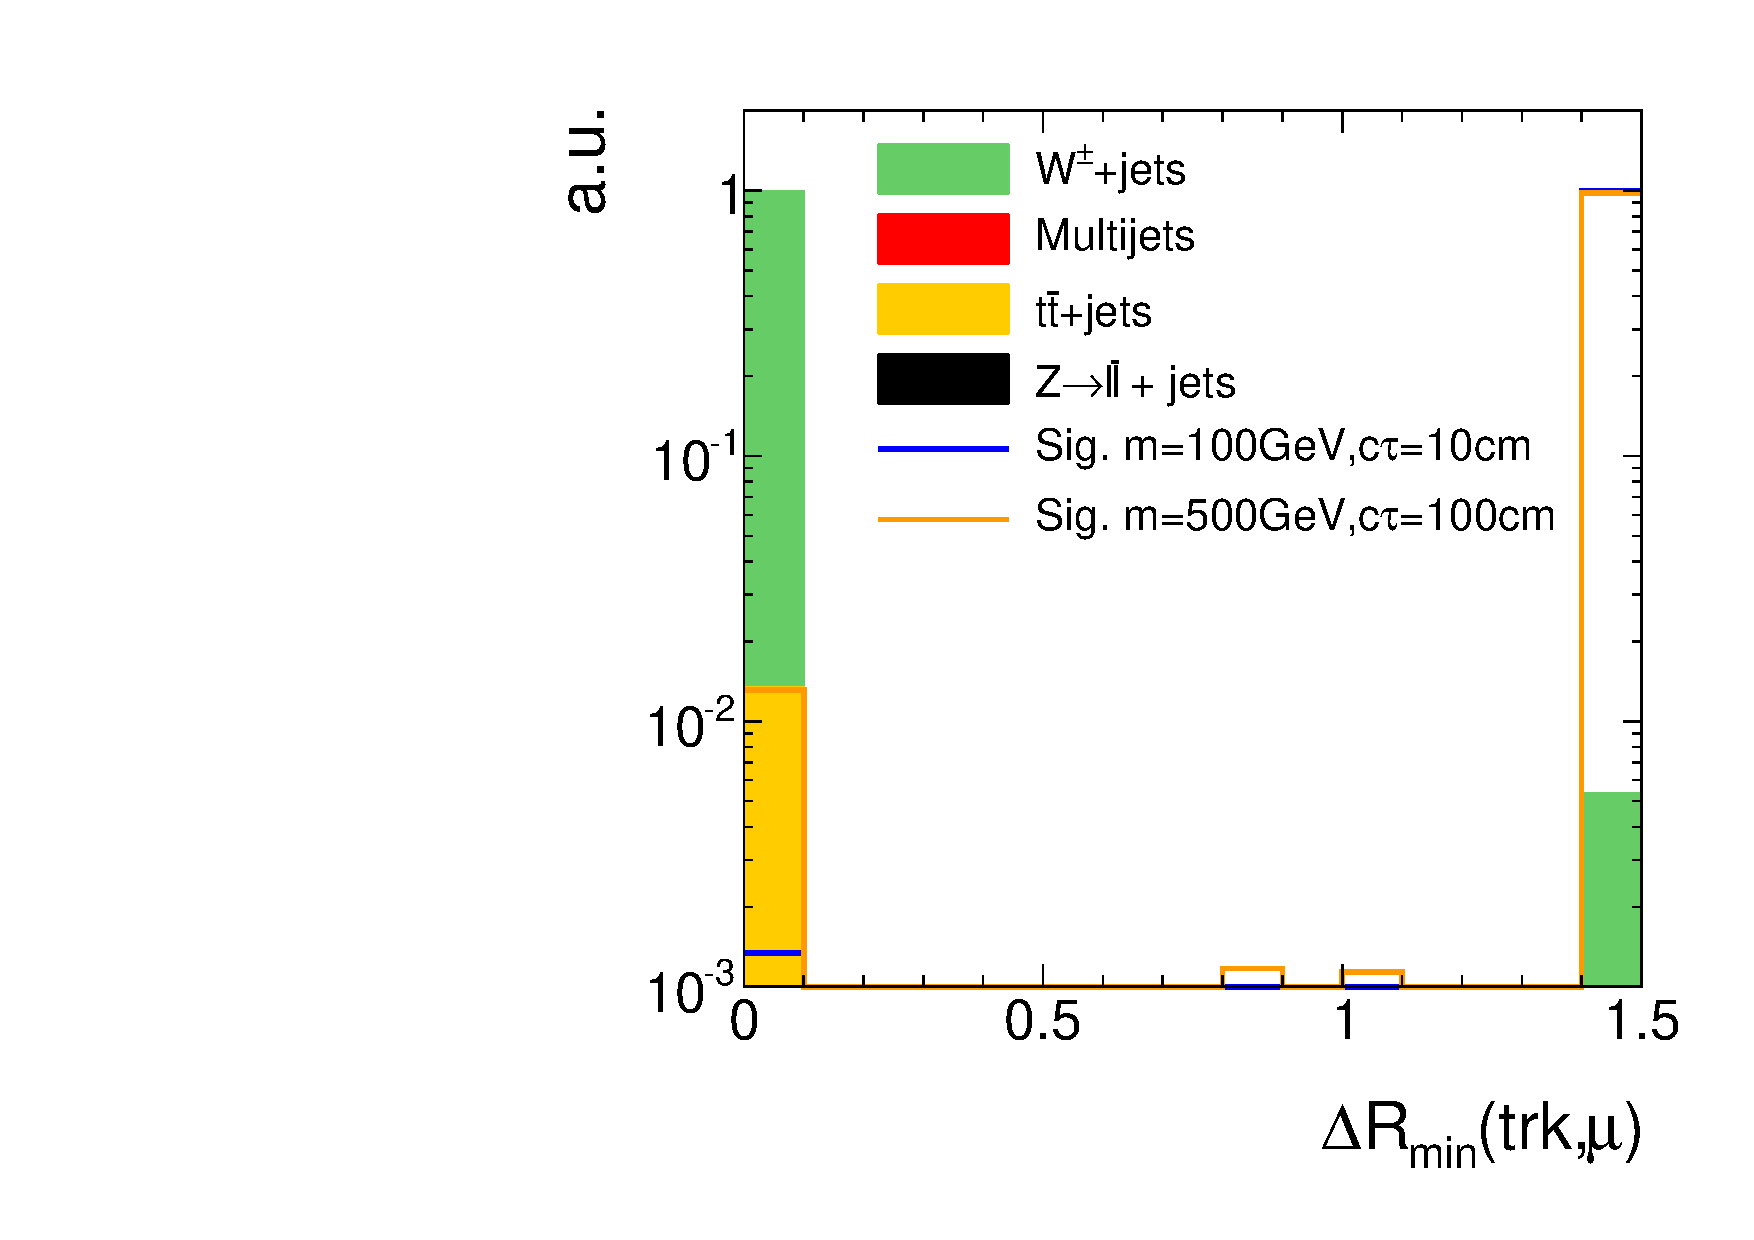
\includegraphics[width=0.49\textwidth]{figures/analysis/AnalysisSelection/htrackdRminMuon_log.pdf}\\

    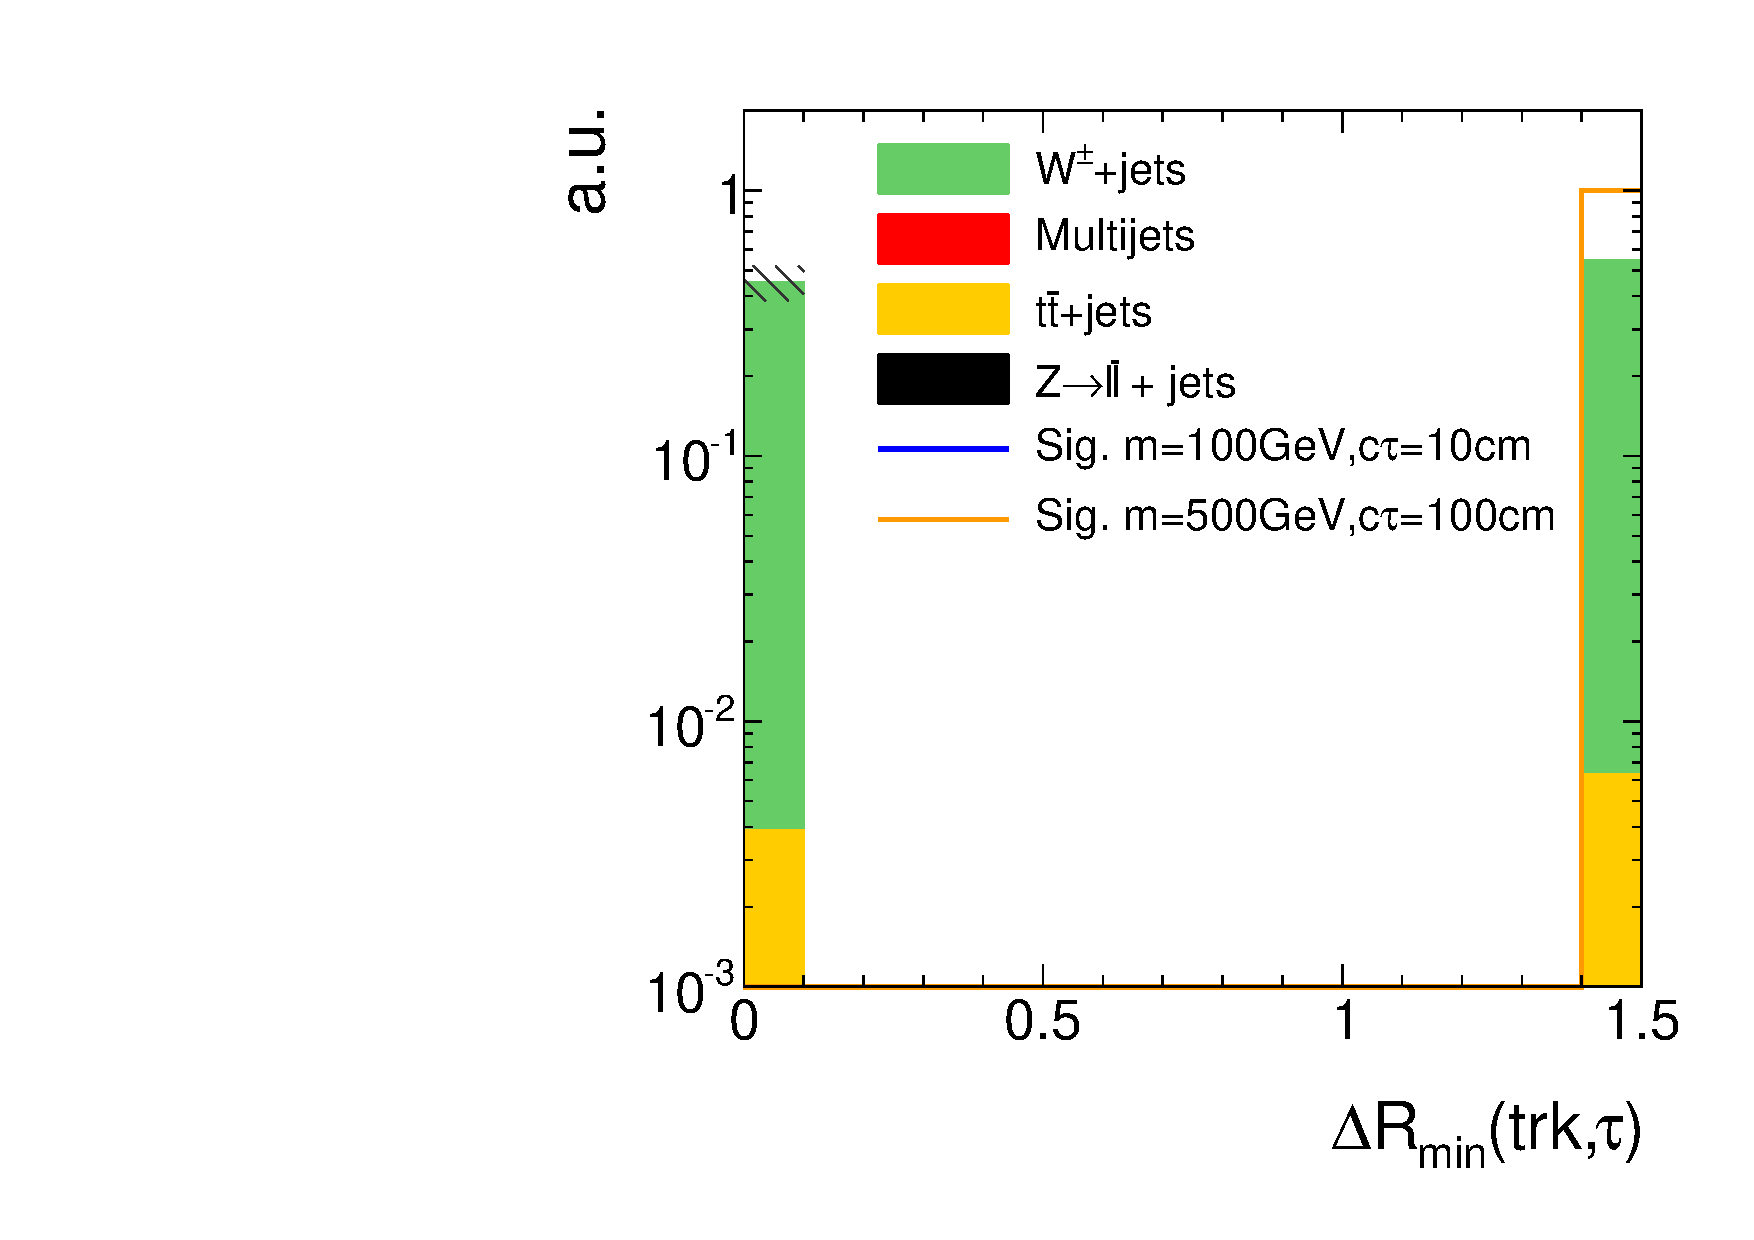
\includegraphics[width=0.49\textwidth]{figures/analysis/AnalysisSelection/htrackdRminTau_log.pdf}
    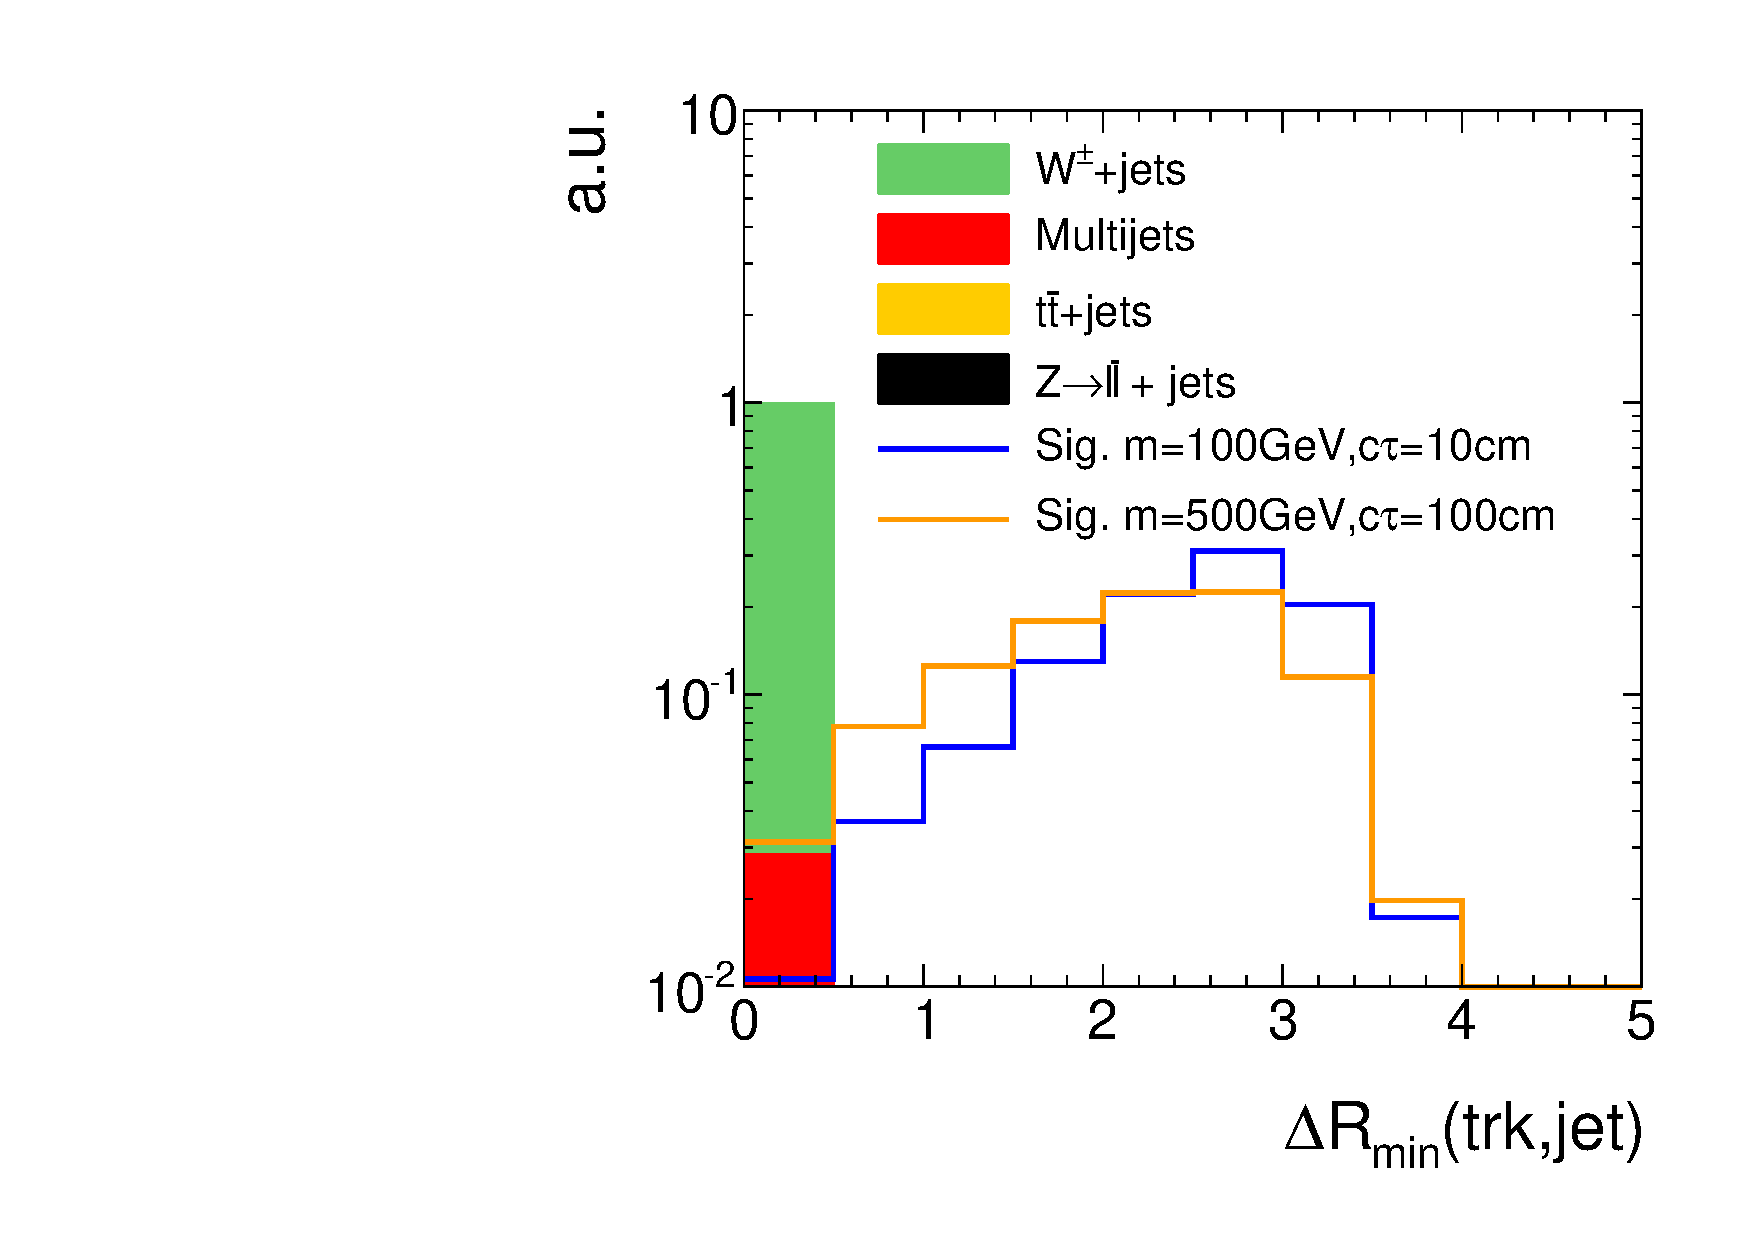
\includegraphics[width=0.49\textwidth]{figures/analysis/AnalysisSelection/htrackdRminJet_log.pdf}
  \end{tabular}
  \caption{The minimum $\Delta R$ between the candidate track and a reconstructed electron (top left), muon (top right), tau (bottom left) or jet (bottom right) 
           after the event-based selection and the high-quality, kinematic and lepton/jet veto selection of the candidate track selection but without the one shown in the corresponding plot (``N-1 plot''). 
           The last bin contains all events where the candidate track has a $\Delta R_{\text{min}}$ larger than 1.5 or 5.0 to the next lepton or jet respectively. 
           Events with no respective lepton or jet are also contained in the last bin.}
  \label{fig:TrackdRmin}
  \vspace{25pt}
\end{figure}

Unfortunately, the lepton veto selection cuts are less effective in some of the detector directions.
For example, the reconstruction of an electron easily fails in the direction of a dead ECAL cell.
This reduces the discrimination power of the electron veto.
For this reason, tracks that point towards dead or noisy ECAL cells are rejected.
A general list of dead and noisy ECAL cells is provided centrally by the CMS collaboration.
Further dead cells were identified within a study in~\cite{bib:CMS:DT_Thesis,bib:CMS:DT_8TeV_AN} resulting in a total number of 1234 dead or noisy ECAL channels (which is about 1.6\% of all ECAL crystals). 
These are illustrated in Fig.~\ref{fig:DeadECALmap} showing a map of all ECAL channels not considered in the search.


Additionally, tracks that point towards intermodule gaps of ECAL cells or to the ECAL barrel endcap gap at $1.42<|\eta|<1.65$ are rejected.
A list of the ECAL intermodule gaps, which is supplied centrally by CMS, is given in Table~\ref{tab:IntermoduleGaps}.

\begin{figure}[!t]
  \vspace{10pt}
  \centering 
  \begin{tabular}{c}
    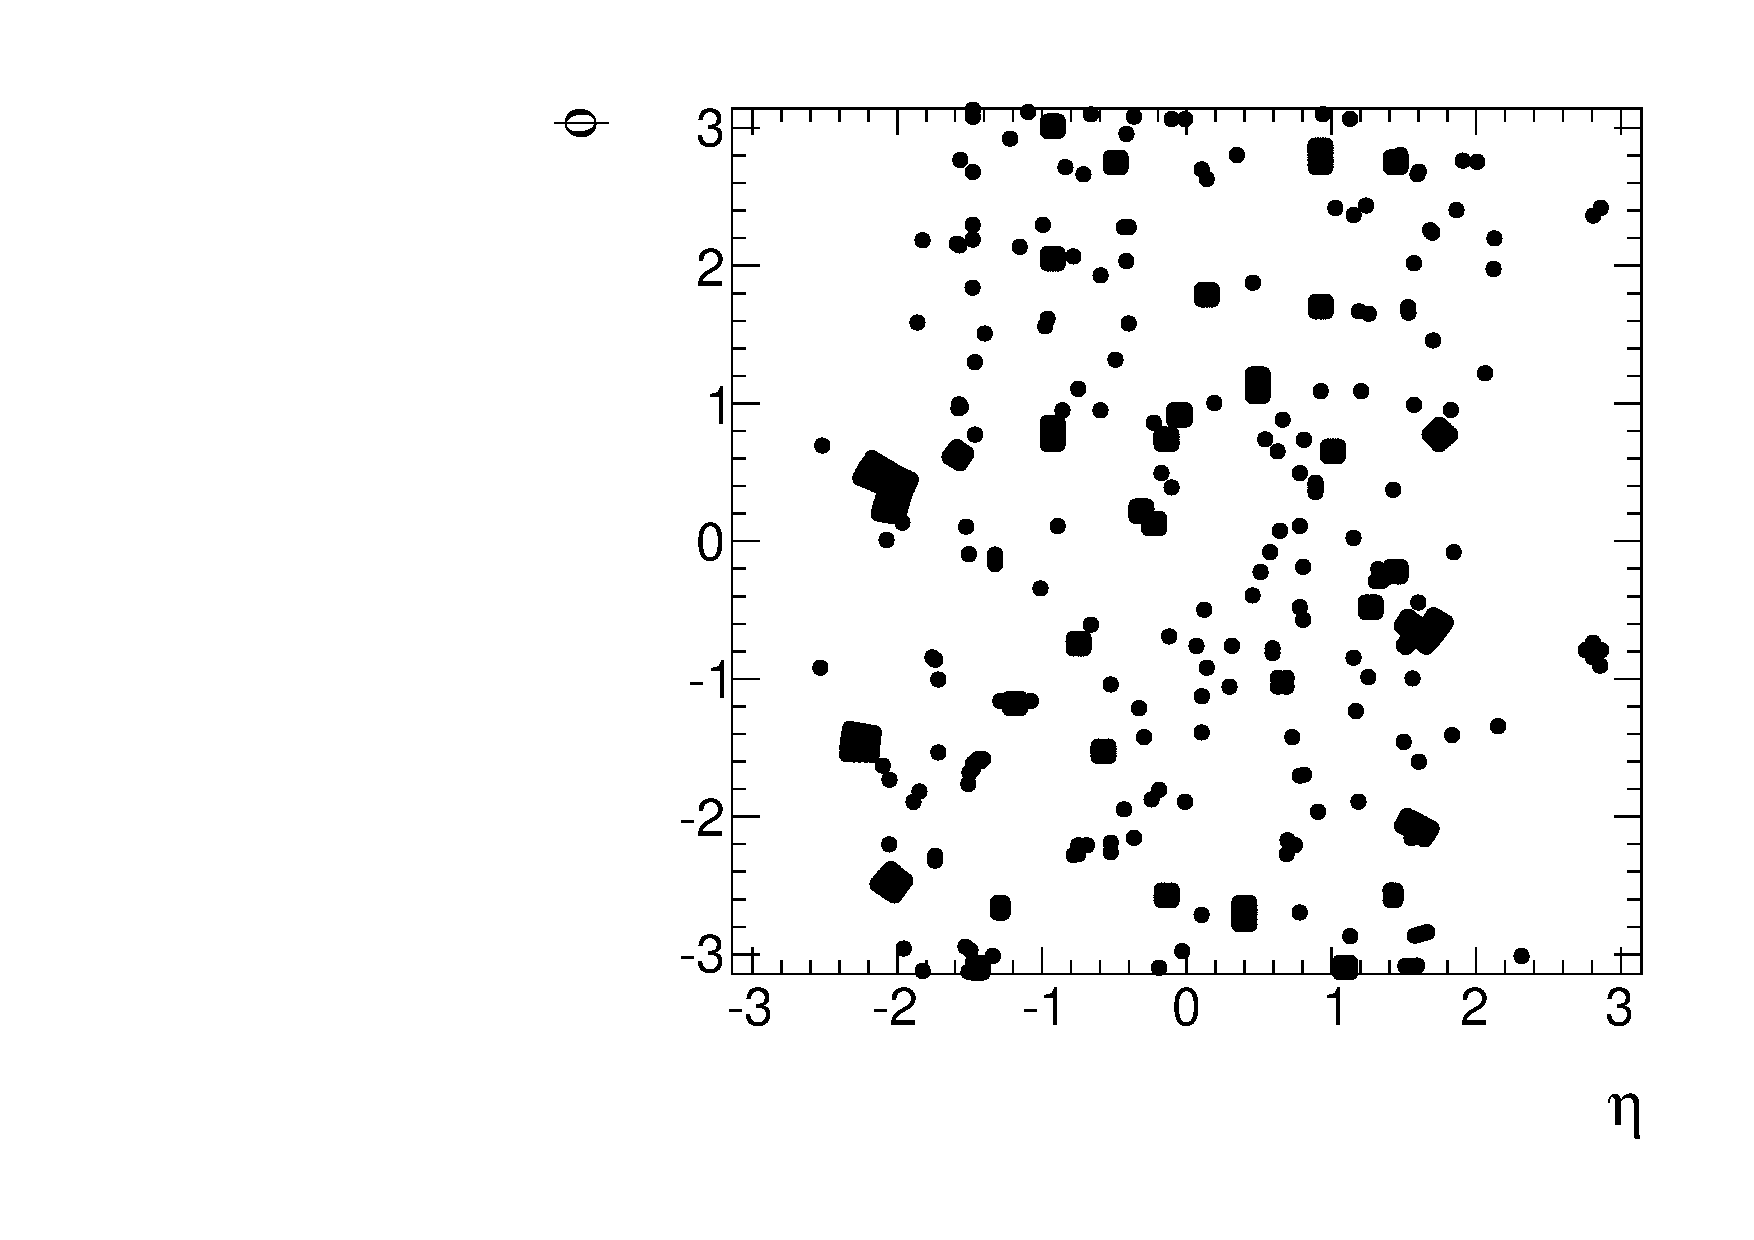
\includegraphics[width=0.49\textwidth]{figures/analysis/AnalysisSelection/DeadECALMap2.pdf}
  \end{tabular}
  \caption{Visualisation of dead and noisy ECAL cells in the detector $\phi - \eta$ plane according to~\cite{bib:CMS:DT_Thesis,bib:CMS:DT_8TeV_AN}.
           The radius of the dots correspond to $\Delta R=0.05$.}
  \label{fig:DeadECALmap}
  \vspace{10pt}
\end{figure}




The muon reconstruction is less efficient for muons in detector regions with bad cathode strip chambers (CSC).
These bad chambers are also identified centrally by the CMS collaboration and their $\eta$ and $\phi$ values are visualised in Fig.~\ref{fig:BadCSCMap}.
Thus, also tracks pointing towards these regions within a distance of $\Delta R<0.25$ are rejected.

\renewcommand{\arraystretch}{1.5}
\begin{table}[!b]
%\vspace{10pt}
\centering
\caption{Intermodule ECAL gaps.}
\label{tab:IntermoduleGaps}
\makebox[0.99\textwidth]{
\begin{tabular}{c}
\multicolumn{1}{c}{} \\
\toprule
$\eta$-ranges     \\
\midrule
 -1.14018  $< \eta <$ -1.1439 \\
-0.791884  $< \eta <$ -0.796051 \\
-0.44356   $< \eta <$  -0.447911 \\
0.00238527 $< \eta <$ -0.00330793 \\
0.446183   $< \eta <$ 0.441949 \\
0.793955   $< \eta <$ 0.789963 \\
1.14164    $< \eta <$ 1.13812 \\
\bottomrule
\multicolumn{1}{c}{} \\
\end{tabular}}
\vspace{50pt}
\end{table}  

\begin{figure}[!b]
  \centering 
  \begin{tabular}{c}
    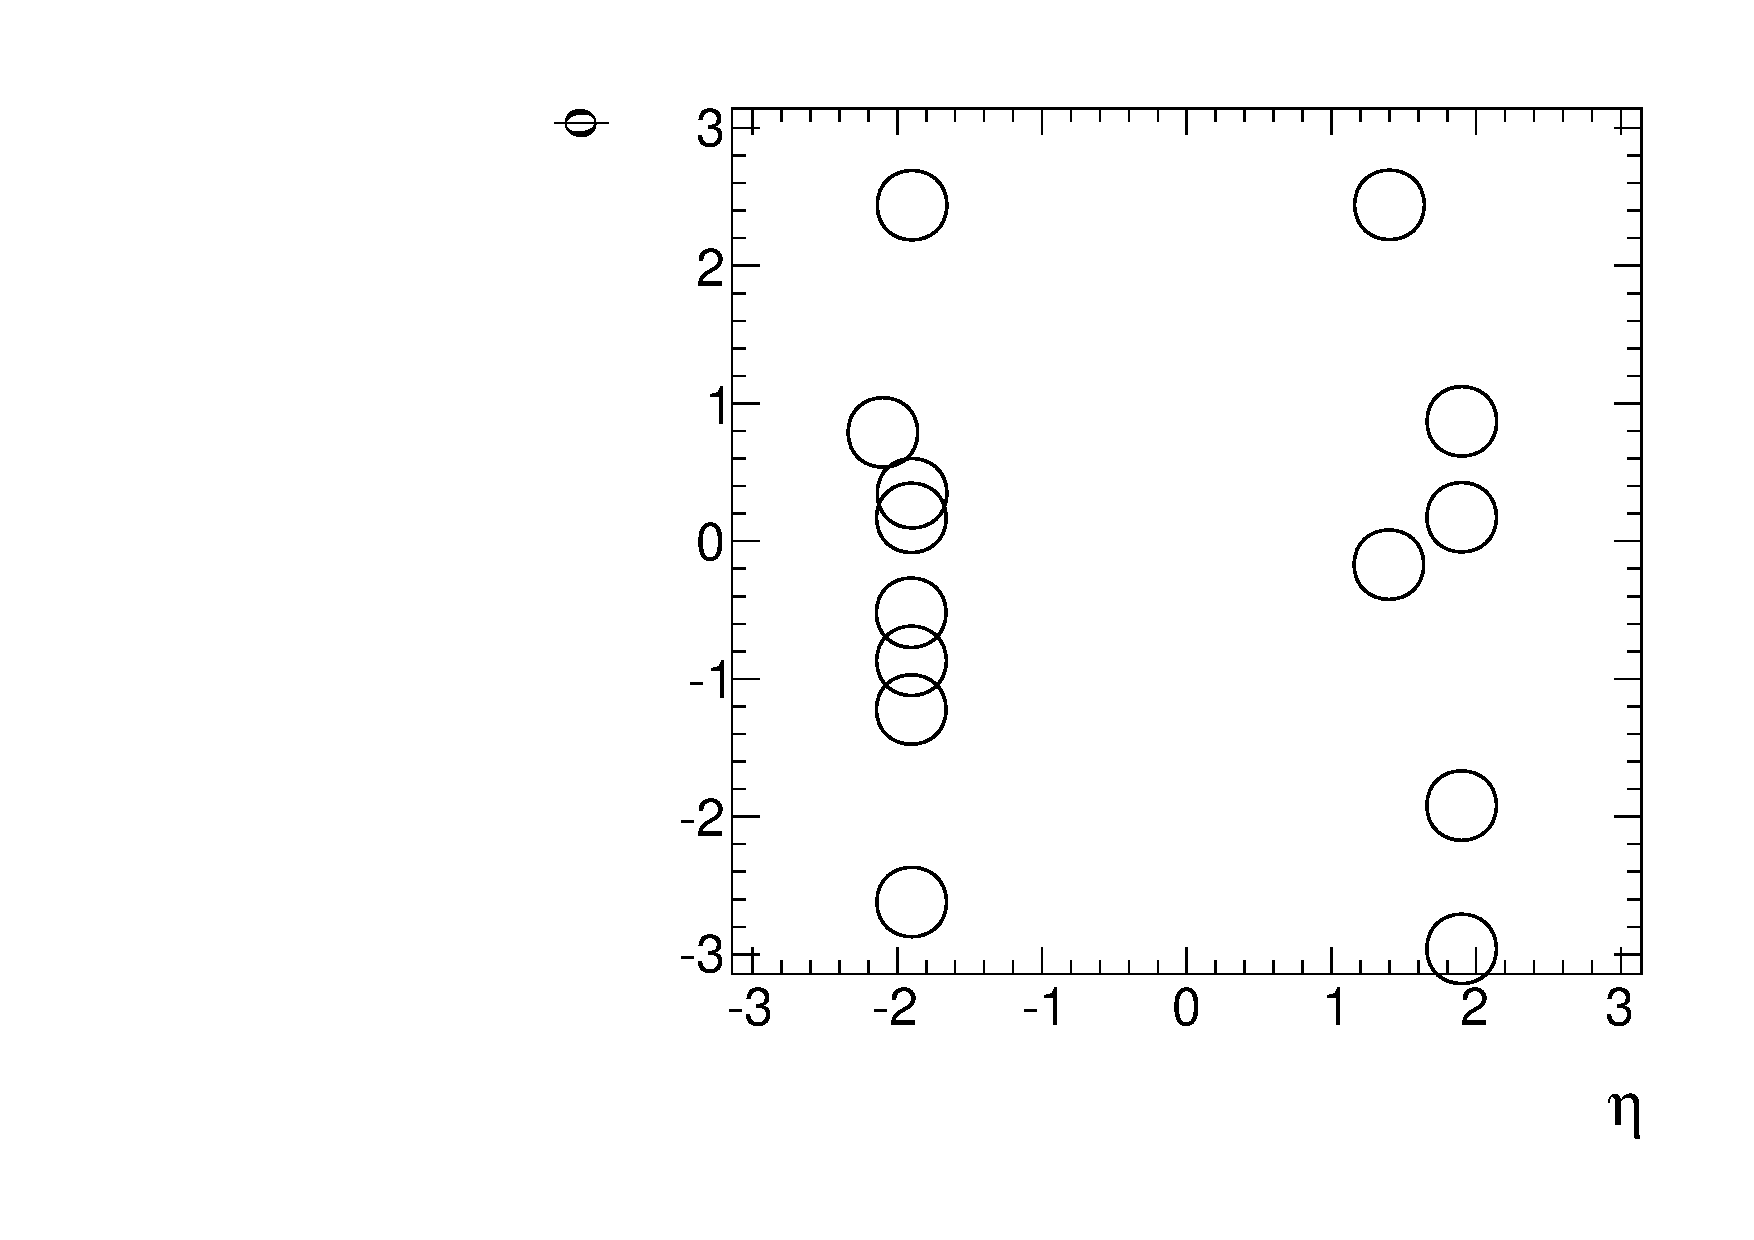
\includegraphics[width=0.49\textwidth]{figures/analysis/AnalysisSelection/BadCSCMap2.pdf}
  \end{tabular}
  \caption{Visualisation of the excluded region by the bad cathode strip chamber veto in the detector $\phi - \eta$.}
  \label{fig:BadCSCMap}
\vspace{30pt}
\end{figure}

To summarise, tracks pointing towards detector regions, that are not working properly or where the lepton reconstruction efficiencies are reduced, are vetoed as follows:
\begin{itemize}
\renewcommand{\labelitemi}{\footnotesize{\ding{118}}}
\item Veto tracks within a cone of $\Delta R<0.05$ to a dead or noisy ECAL cell (visualised in Fig.~\ref{fig:DeadECALmap}).
\item Veto tracks that point towards the direction of the ECAL intermodule gap listed in Table~\ref{tab:IntermoduleGaps}.
\item Veto tracks that point towards a bad CSC within $\Delta R<0.25$ (visualised in Fig.~\ref{fig:BadCSCMap}).
\item Veto tracks that point towards the region between ECAL barrel and endcap at $1.42<|\eta|<1.65$\\
\end{itemize}



Finally, two further characteristics of chargino tracks are exploited.
As the chargino is produced in a very clean environment (no further particles around the chargino is expected), the isolation of the track can discriminate signal against background events.
Furthermore, for charginos decaying inside the tracker there is no associated energy deposition in the calorimeters in the direction of the track.
This is a very pronounced characteristics of signal tracks for short chargino lifetimes. 
The resulting selection cuts are as follows
\begin{itemize}
\renewcommand{\labelitemi}{\footnotesize{\ding{118}}}
\item No further substantial track activity is allowed in a cone of $\Delta R < 0.3$ around the candidate track: \mbox{$\sum \limits_{\Delta R < 0.3} \pt^{\text{trk}}/\pt^{\text{cand}} - 1 < 0.1$} (the subtraction by $1$ corresponds to the contribution of the candidate track itself)
\item No large calorimeter energy deposits (ECAL+HCAL) in a cone of $\Delta R < 0.5$ around the track: \mbox{$\ecalo<5\gev$}.
\end{itemize}
The discrimination power of these two variables is shown in Fig.~\ref{fig:TrackIso_Ecalo_After_Preselection}.
\begin{figure}[!b]
  \centering 
  \begin{tabular}{c}
    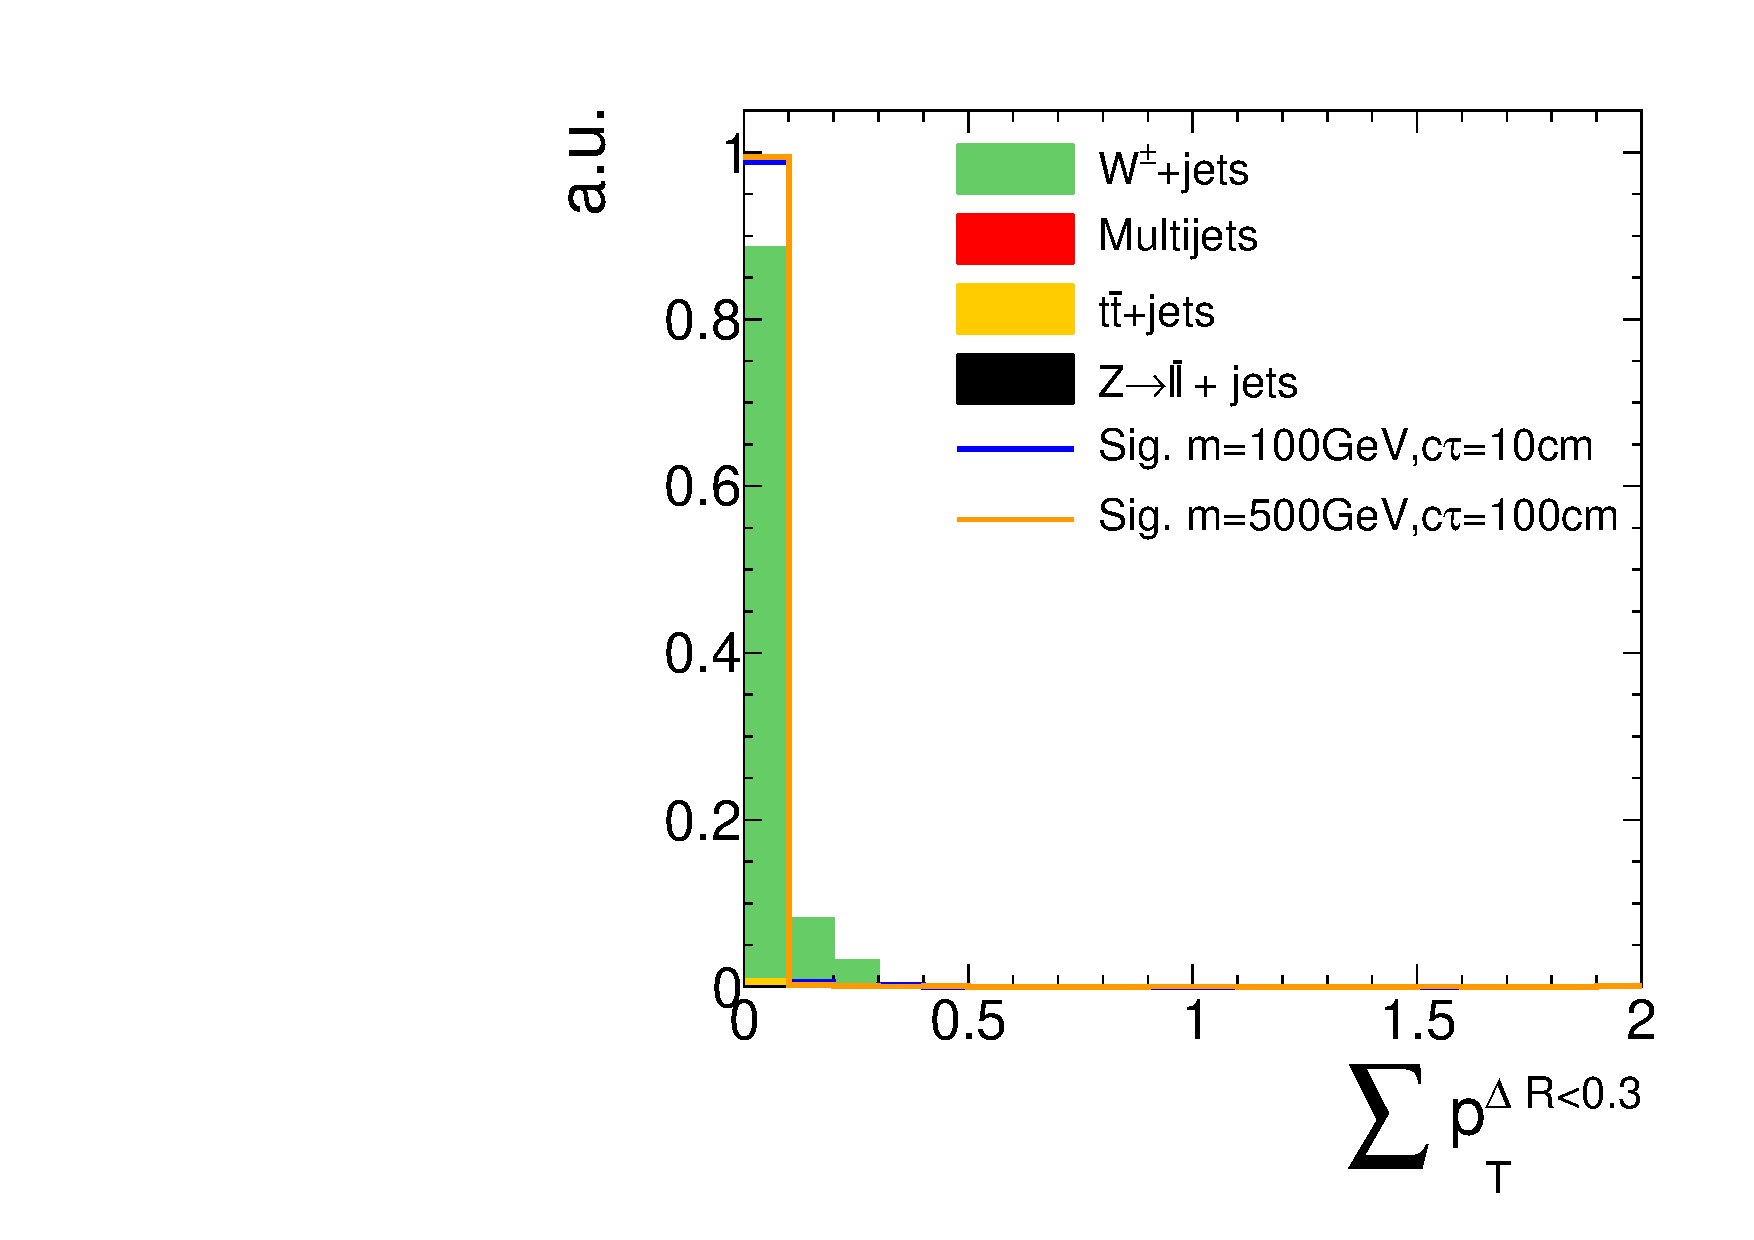
\includegraphics[width=0.49\textwidth]{figures/analysis/AnalysisSelection/chiTracksCandidateSelectionTrigger_2Signals_FullBkg/htrackIsolation_lin.pdf}
    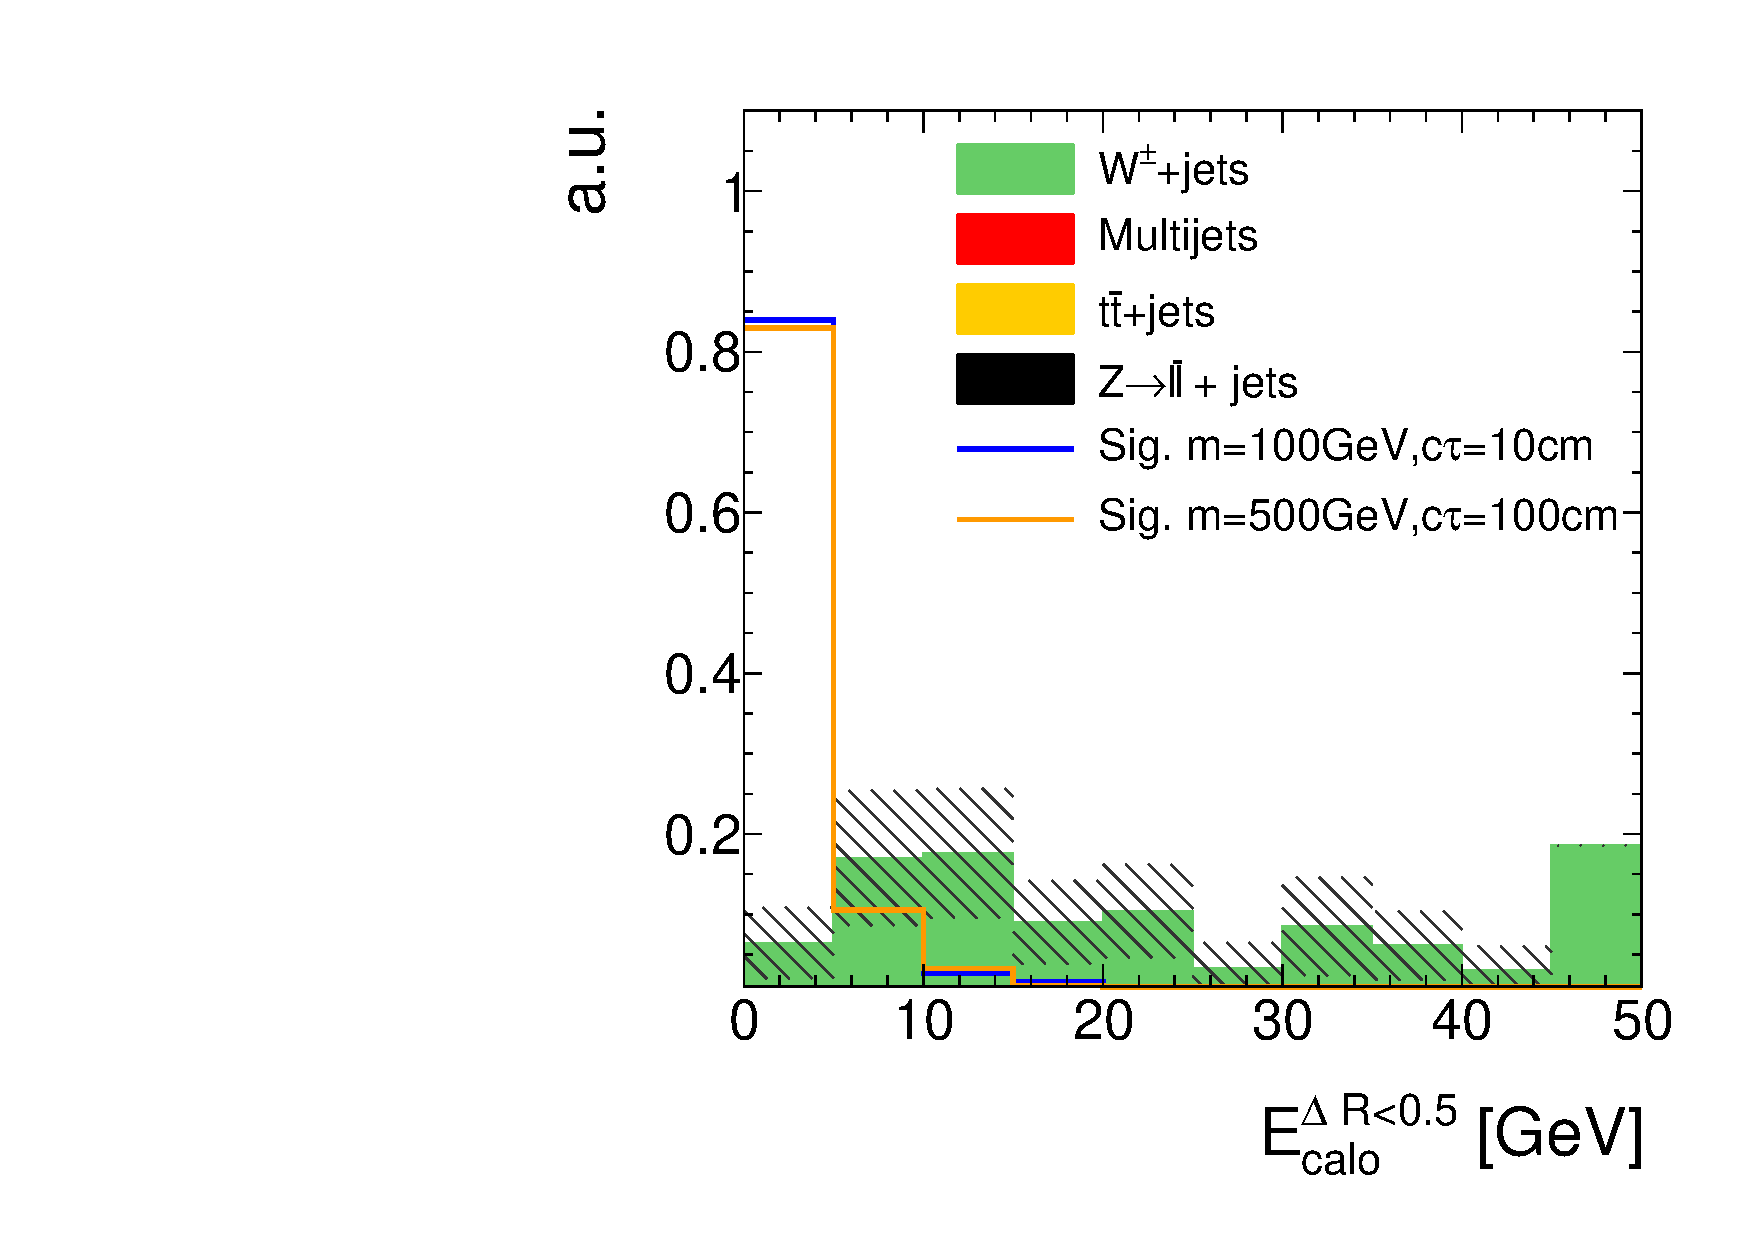
\includegraphics[width=0.49\textwidth]{figures/analysis/AnalysisSelection/chiTracksCandidateSelectionTrigger_2Signals_FullBkg/htrackCaloIsolation_lin.pdf}
  \end{tabular}
  \caption{Track isolation (left) and calorimeter energy deposits (right) of the candidate track after the full previous selection. 
           All events with a track isolation or a calorimeter energy deposit larger than the range shown in the figures are contained in the last bin.}
  \label{fig:TrackIso_Ecalo_After_Preselection}
\end{figure}
For even higher chargino lifetimes $\ctau > 100\cm$, the calorimeter isolation requirement starts rejecting signal events because the charginos reach the calorimeters.

As emphasised before, this analysis aims at being sensitive especially on shorter lifetimes.
Still, in order to allow for charginos decaying at any position in the tracker, no explicit selection cut on the number of missing outer hits is required.

Events are selected if they at least contain one track fulfilling all candidate track selection requirements.
An overview over the full analysis preselection is given in Table~\ref{tab:SummaryCuts}. 
\renewcommand{\arraystretch}{1.40}
\begin{table}[!h]
\vspace{5pt}
\centering
\caption{Summary and categorisation of the analysis selection.}
\label{tab:SummaryCuts}
\resizebox{\textwidth}{!}{
\begin{tabular}{l|l|l}
\multicolumn{3}{c}{} \\
\toprule
   
\multirow{3}{*}{Trigger}                                       &  \multicolumn{2}{l}{HLTMonoCentralPFJet80\_PFMETnoMu95\_NHEF0p95 }\\
                                                               &  \multicolumn{2}{l}{HLTMonoCentralPFJet80\_PFMETnoMu105\_NHEF0p95}\\
                                                               &  \multicolumn{2}{l}{HLT\_MET120\_HBHENoiseCleaned }\\\midrule

\multirow{4}{*}{\makecell[l]{Event-based \\ selection}}        &  \multirow{2}{*}{Trigger selection}   & \makecell[l]{$\ptfirstjet>110\gev$ \hfill with $|\eta_{\text{\nth{1}jet}}|<2.4$,  \\
                                                                                                                   \hfill $\text{CHF}_{\text{\nth{1}jet}}>0.2$, \\
                                                                                                                   \hfill $\text{CEF}_{\text{\nth{1}jet}}<0.5$, \\
                                                                                                                   \hfill $\text{NHF}_{\text{\nth{1}jet}}<0.7$, \\
                                                                                                                   \hfill $\text{NEF}_{\text{\nth{1}jet}}<0.7$\phantom{,}} \\
                                                               &                                       & $\met>100\gev$                                                  \\\cmidrule{2-3}
                                                               &  \multirow{2}{*}{QCD suppression}      & \makecell[l]{$\Delta\phi_{\text{max}} \left( \text{jet}_i, \text{jet}_j  \right)<2.7$  for all jets with \\ \hfill $\pt>20\gev$, $|\eta|<4.5$}\\
                                                               &                                       & \makecell[l]{$\Delta\phi_{\text{max}} \left( \text{jet}_{i}, \met  \right)>0.5$  for two leading jets}\\

\midrule

\multirow{18}{*}{\makecell[l]{Candidate track\\ selection}}      &  \multicolumn{2}{l}{$\geq1$ track that fulfils the following criteria:}\\\cmidrule{2-3}

                                                              &  \multirow{4}{*}{Good quality selection}   & high-purity as defined in~\cite{bib:CMS:Tracking_2010} \\
                                                              &                                            & $N_{\text{miss}}^{\text{middle/inner}}=0$\\
                                                              &                                            & $|d0|<0.02\cm$\\
                                                              &                                            & $|dz|<0.5\cm$\\\cmidrule{2-3}

                                                              &  \multirow{2}{*}{Kinematic selection}      & $|\eta|<2.1$ \\
                                                              &                                            & $\pt>20\gev$ \\\cmidrule{2-3}

                                                              &  \multirow{8}{*}{Lepton/jet veto}          & No muon within $\Delta R<0.15$ \\
                                                              &                                            & No electron within $\Delta R<0.15$ \\
                                                              &                                            & No tau within $\Delta R<0.15$ \\
                                                              &                                            & No jet within $\Delta R<0.5$ \\
                                                              &                                            & No dead/noisy ECAL cell within $\Delta R<0.05$  \\
                                                              &                                            & Not within an ECAL intermodule gap  \\
                                                              &                                            & Not within $1.42<|\eta|<1.65$ \\
                                                              &                                            & Not within $\Delta R<0.25$ to a bad CSC \\\cmidrule{2-3}

                                                              &  \multirow{2}{*}{Isolation selection}      & $\sum \limits_{\Delta R < 0.3} \pt^{\text{trk}}/\pt^{\text{cand}} -1  < 0.1$ \\
                                                              &                                            & $\ecalo<5\gev$ \\


\bottomrule
\end{tabular}}
\vspace{5pt}
\end{table}
The event yields after the selections of each of the categories from Table~\ref{tab:SummaryCuts} are listed in Table~\ref{tab:CutflowALL} for the available simulated background samples, some exemplary simulated signal models and for observed data.
The discrepancies between data and simulation after the full preselection is stemming from three effects.
First, the simulated yield is highly uncertain because of large event weights ($\sim 15$).
Second, not all relevant background samples were available (\eg \ZInvJets sample), leading to a lower prediction in simulation.
Third, simulation is not expected to describe the here selected events (lepton/jet veto) very well.
This emphasises once more the need for data-driven background estimation methods.
Detailed event yield tables can be found in Appendix~\ref{app:cutflow}.\\
%%%%%%%%%%%%%%%%%%%%%%%%
\renewcommand{\arraystretch}{1.5}
\begin{sidewaystable}[!h]
\centering
\caption{Event yields in simulation and data after the selections of each of the categories from Table~\ref{tab:SummaryCuts}}
\label{tab:CutflowALL}
\makebox[0.99\textwidth]{
\begin{tabular}{|l|c|c|c|c|c|c|c|c|c|}
\multicolumn{10}{c}{} \\
\toprule
                            & \multicolumn{4}{c|}{Simulated background samples}      & \multicolumn{4}{c|}{Simulated signal samples}  & Data         \\
\midrule
\multirow{2}{*}{Selection}  & \multirow{2}{*}{\WJets} & \multirow{2}{*}{\ttbarJets} & \multirow{2}{*}{\Zlep} & \multirow{2}{*}{Multijet} & m\shorteq100GeV     & m\shorteq100GeV      & m\shorteq500GeV    & m\shorteq500GeV  & MET      \\
                            &                         &                             &                        &       & $c\tau$\shorteq10\cm & $c\tau$\shorteq100\cm & $c\tau$\shorteq10\cm & $c\tau$\shorteq100\cm &  data            \\
\midrule
After skim                                                                                & 9.16 $\cdot10^{7 }$ & 1.04 $\cdot10^{6 }$ & 2.21 $\cdot10^{7 }$ & 1.38 $\cdot10^{11}$ & 3.41 $\cdot10^{5 }$ & 3.41 $\cdot10^{5 }$ & 3.46 $\cdot10^{2 }$ & 3.46 $\cdot10^{2 }$ & 1.07 $\cdot10^{7 }$ \\
Event-based selection:                                                                    
& & & & & & & & & \\
Trigger                                                                                   & 4.31 $\cdot10^{6 }$ & 1.15 $\cdot10^{5 }$ & 4.23 $\cdot10^{3 }$ & 4.32 $\cdot10^{6 }$ & 1.55 $\cdot10^{4 }$ & 1.49 $\cdot10^{4 }$ & 46.2 & 46.2 & 1.07 $\cdot10^{7 }$ \\
Trigger selection                                                                         & 1.89 $\cdot10^{6 }$ & 5.31 $\cdot10^{4 }$ & 6.26 $\cdot10^{2 }$ & 9.63 $\cdot10^{5 }$ & 1.09 $\cdot10^{4 }$ & 9.83 $\cdot10^{3 }$ & 36.3 & 35.7 & 3.94 $\cdot10^{6 }$ \\
QCD suppression                                                                           & 1.11 $\cdot10^{6 }$ & 6.76 $\cdot10^{3 }$ & 1.32 $\cdot10^{2 }$ & 9.55 $\cdot10^{3 }$ & 7.90 $\cdot10^{3 }$ & 6.98 $\cdot10^{3 }$ & 27.6 & 27.1 & 1.38 $\cdot10^{6 }$ \\
Track-based selection:                                                                    
& & & & & & & & & \\
Good quality selection                                                                    & 1.07 $\cdot10^{6 }$ & 6.63 $\cdot10^{3 }$ & 1.32 $\cdot10^{2 }$ & 9.55 $\cdot10^{3 }$ & 2.80 $\cdot10^{3 }$ & 5.38 $\cdot10^{3 }$ & 5.07  & 20.0 & 1.30 $\cdot10^{6 }$ \\
Kinematic selection                                                                       & 8.14 $\cdot10^{5 }$ & 5.63 $\cdot10^{3 }$ & 1.32 $\cdot10^{2 }$ & 5.48 $\cdot10^{3 }$ & 2.54 $\cdot10^{3 }$ & 4.93 $\cdot10^{3 }$ & 4.73  & 18.9 & 9.51 $\cdot10^{5 }$ \\
Lepton/jet veto                                                                           & 5.02 $\cdot10^{2 }$ & 5.88  & 0  & 0  & 1.99 $\cdot10^{3 }$ & 3.67 $\cdot10^{3 }$ & 3.83  & 15.0  & 616 \\
Isolation selection                                                                       & 31.9  & 0.67  & 0  & 0  & 1.67 $\cdot10^{3 }$ & 3.04 $\cdot10^{3 }$ & 3.39  & 12.6  & 119  \\
\bottomrule
\end{tabular}}
\end{sidewaystable}
%\end{landscape}

%\clearpage
Given the presented signal candidate selection, two variables remain that are highly discriminating:
The transverse momentum \pt and the energy release per path length \dedx of the candidate track.
In this analysis, the Asymmetric Smirnov discriminator \ias is used to enhance the discriminating power of \dedx (see Section~\ref{sec:Ias} for the definition and a detailed explanation of \ias).
In Fig.~\ref{fig:PtAndIasAfterFullPreselection}, the distribution of the remaining two variables are shown after the selection of signal candidate events.
\begin{figure}[!b]
  \centering 
  \begin{tabular}{c}
    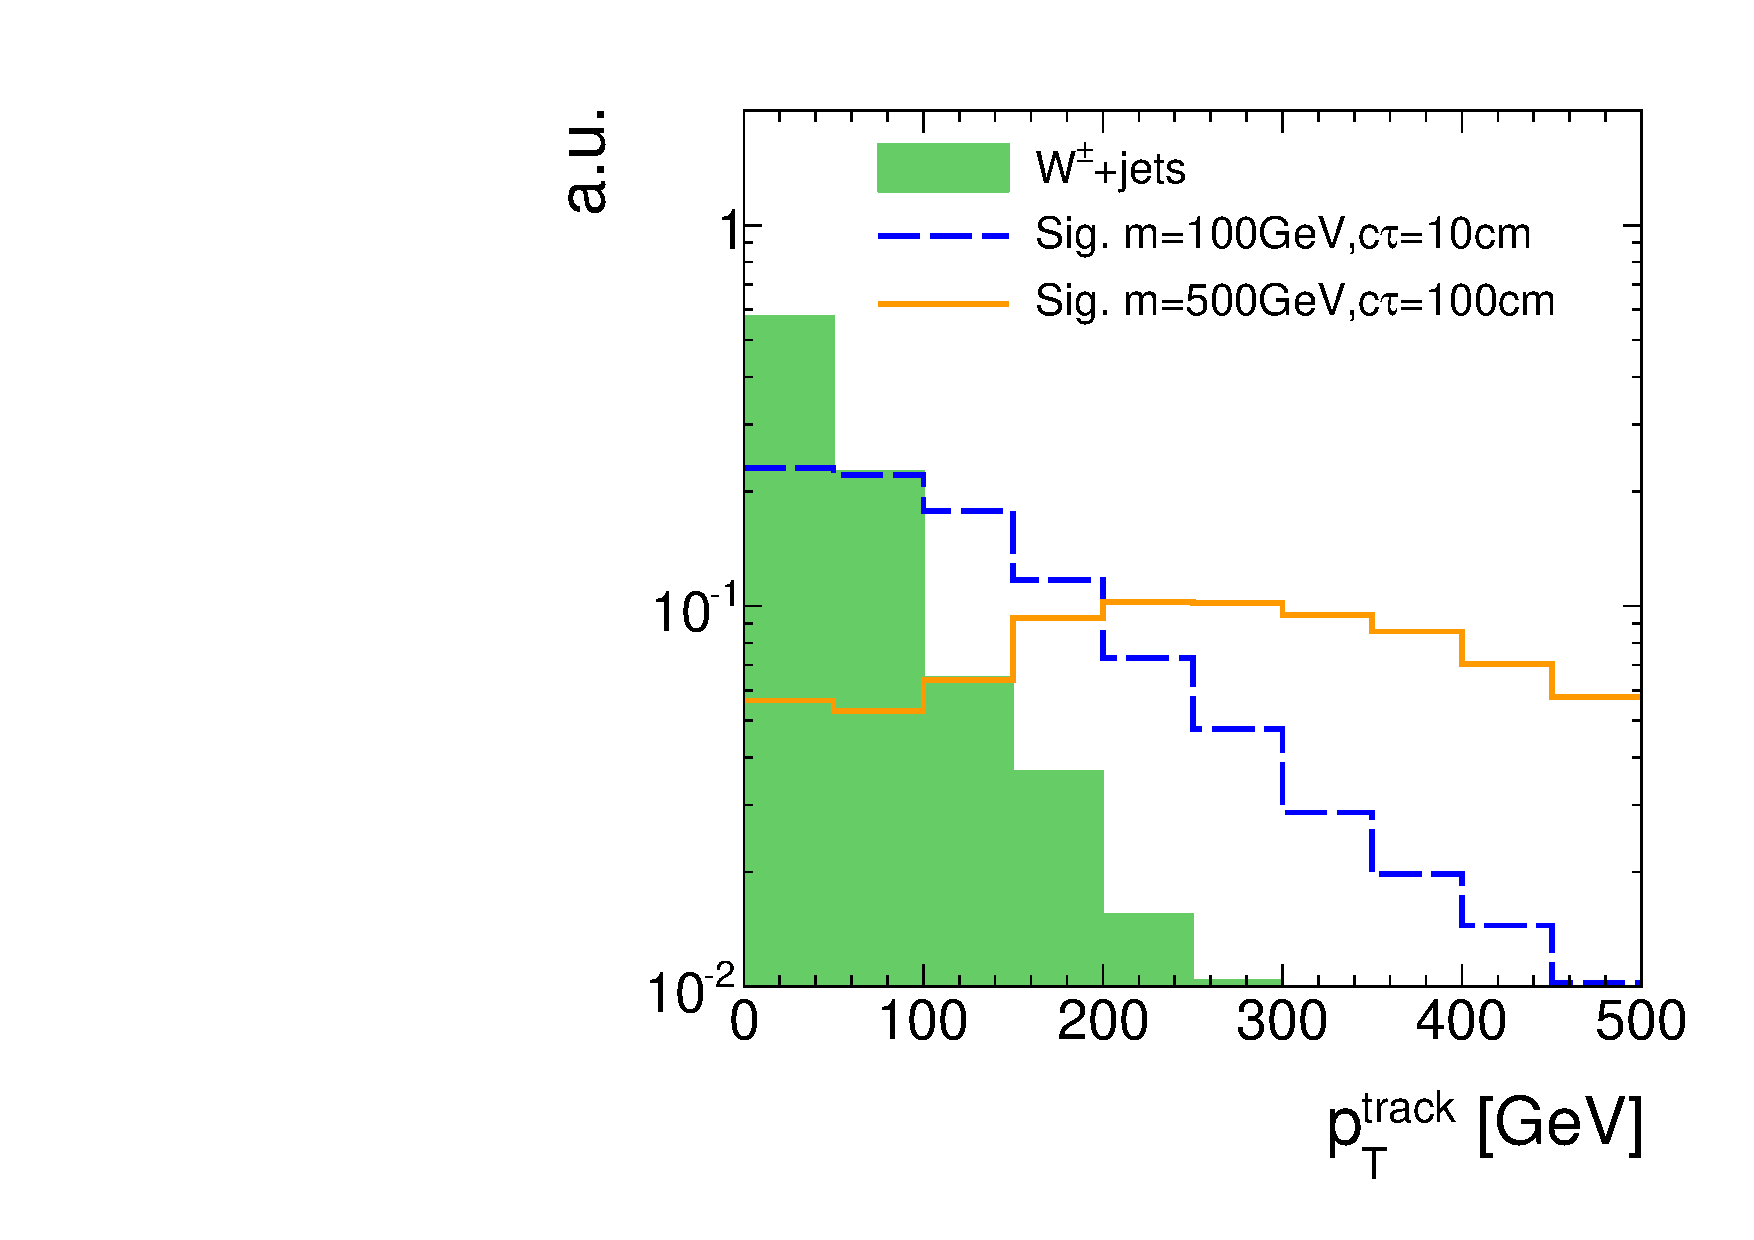
\includegraphics[width=0.49\textwidth]{figures/analysis/AnalysisSelection/chiTracksfullSelectionNoTriggerCuts_Wjets/htrackPtSmallRangeCoarseBinning_log.pdf}
    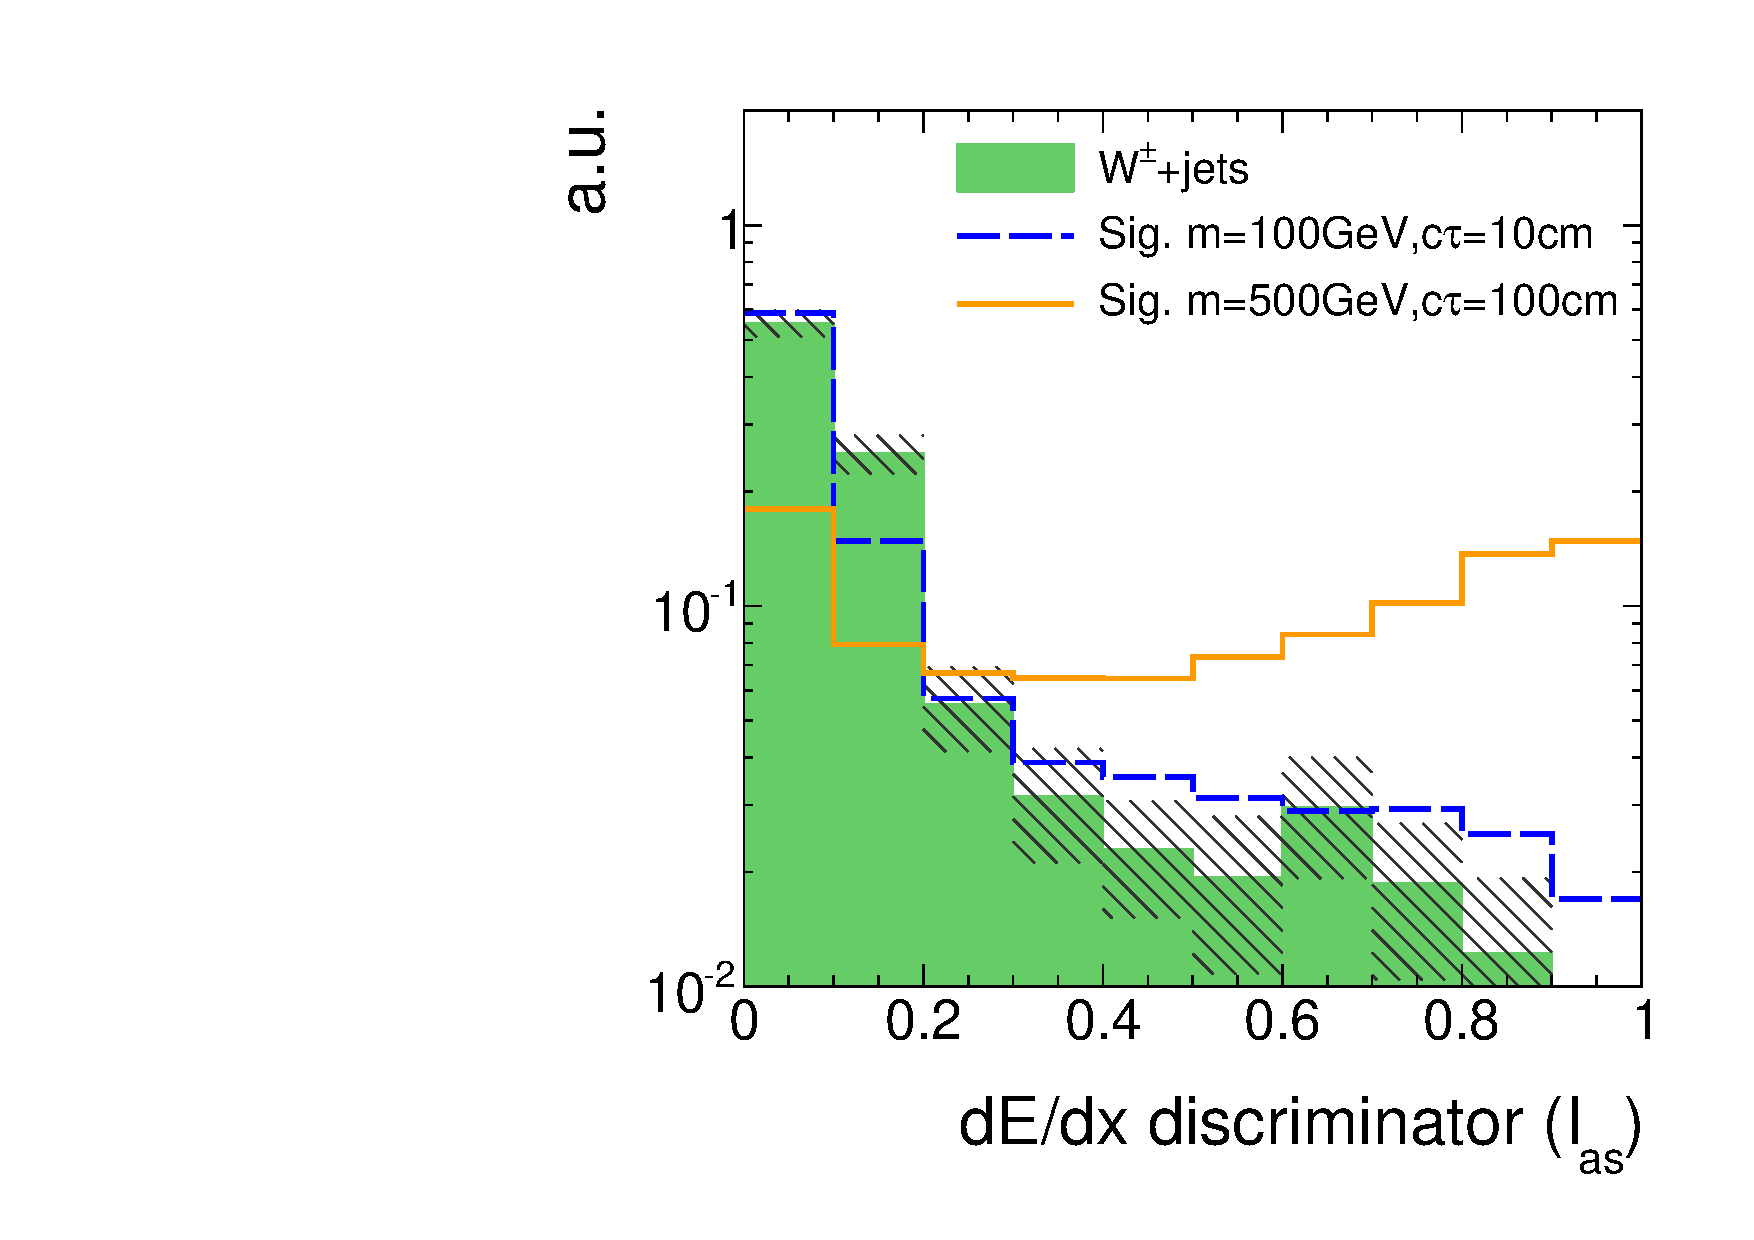
\includegraphics[width=0.49\textwidth]{figures/analysis/AnalysisSelection/chiTracksfullSelectionNoTriggerCuts_Wjets/htrackASmiSmallRange_log.pdf}
  \end{tabular}
  \caption{Candidate track \pt (left) and \ias (right) after the full signal candidate selection for signal and $\WJets$ events. 
           Because of the low statistical precision of the $\WJets$ sample, the trigger selection is not applied.
           }
  \label{fig:PtAndIasAfterFullPreselection}
\end{figure}
These variables are used to optimise the sensitivity of the search.
The optimisation process will be explained in Section~\ref{ch:Optimisation}.
However, before the optimisation can be accomplished, a characterisation and estimation of the background is needed.
This topic will be discussed in the following chapter.



%%%%%%%%%%%%%%%%%%%%%%%%%%%%%%%%%%%%%%%%%%%%%%%%%%%%%%%%%%%%%%%%%%%%%%%%%%%%%%%%%%%%%%%%%%%%%%%%%%%%%%%%%%%%%%%%%%%%%%%%%%%%%%%%%%%%%%%%%%%%%%%%%%%%%%%%%%%%%%%%%%%%%%%%%%%%%%%%%%%%
%%%%%%%%%%%%%%%%%%%%%%%%%%%%%%%%%%%%%%%%%%%%%%%%%%%%%%%%%%%%%%%%%%%%%%%%%%%%%%%%%%%%%%%%%%%%%%%%%%%%%%%%%%%%%%%%%%%%%%%%%%%%%%%%%%%%%%%%%%%%%%%%%%%%%%%%%%%%%%%%%%%%%%%%%%%%%%%%%%%%

